
% Default to the notebook output style

    


% Inherit from the specified cell style.




    
\documentclass[11pt]{article}

    
    
    \usepackage[T1]{fontenc}
    % Nicer default font (+ math font) than Computer Modern for most use cases
    \usepackage{mathpazo}

    % Basic figure setup, for now with no caption control since it's done
    % automatically by Pandoc (which extracts ![](path) syntax from Markdown).
    \usepackage{graphicx}
    % We will generate all images so they have a width \maxwidth. This means
    % that they will get their normal width if they fit onto the page, but
    % are scaled down if they would overflow the margins.
    \makeatletter
    \def\maxwidth{\ifdim\Gin@nat@width>\linewidth\linewidth
    \else\Gin@nat@width\fi}
    \makeatother
    \let\Oldincludegraphics\includegraphics
    % Set max figure width to be 80% of text width, for now hardcoded.
    \renewcommand{\includegraphics}[1]{\Oldincludegraphics[width=.8\maxwidth]{#1}}
    % Ensure that by default, figures have no caption (until we provide a
    % proper Figure object with a Caption API and a way to capture that
    % in the conversion process - todo).
    \usepackage{caption}
    \DeclareCaptionLabelFormat{nolabel}{}
    \captionsetup{labelformat=nolabel}

    \usepackage{adjustbox} % Used to constrain images to a maximum size 
    \usepackage{xcolor} % Allow colors to be defined
    \usepackage{enumerate} % Needed for markdown enumerations to work
    \usepackage{geometry} % Used to adjust the document margins
    \usepackage{amsmath} % Equations
    \usepackage{amssymb} % Equations
    \usepackage{textcomp} % defines textquotesingle
    % Hack from http://tex.stackexchange.com/a/47451/13684:
    \AtBeginDocument{%
        \def\PYZsq{\textquotesingle}% Upright quotes in Pygmentized code
    }
    \usepackage{upquote} % Upright quotes for verbatim code
    \usepackage{eurosym} % defines \euro
    \usepackage[mathletters]{ucs} % Extended unicode (utf-8) support
    \usepackage[utf8x]{inputenc} % Allow utf-8 characters in the tex document
    \usepackage{fancyvrb} % verbatim replacement that allows latex
    \usepackage{grffile} % extends the file name processing of package graphics 
                         % to support a larger range 
    % The hyperref package gives us a pdf with properly built
    % internal navigation ('pdf bookmarks' for the table of contents,
    % internal cross-reference links, web links for URLs, etc.)
    \usepackage{hyperref}
    \usepackage{longtable} % longtable support required by pandoc >1.10
    \usepackage{booktabs}  % table support for pandoc > 1.12.2
    \usepackage[inline]{enumitem} % IRkernel/repr support (it uses the enumerate* environment)
    \usepackage[normalem]{ulem} % ulem is needed to support strikethroughs (\sout)
                                % normalem makes italics be italics, not underlines
    

    
    
    % Colors for the hyperref package
    \definecolor{urlcolor}{rgb}{0,.145,.698}
    \definecolor{linkcolor}{rgb}{.71,0.21,0.01}
    \definecolor{citecolor}{rgb}{.12,.54,.11}

    % ANSI colors
    \definecolor{ansi-black}{HTML}{3E424D}
    \definecolor{ansi-black-intense}{HTML}{282C36}
    \definecolor{ansi-red}{HTML}{E75C58}
    \definecolor{ansi-red-intense}{HTML}{B22B31}
    \definecolor{ansi-green}{HTML}{00A250}
    \definecolor{ansi-green-intense}{HTML}{007427}
    \definecolor{ansi-yellow}{HTML}{DDB62B}
    \definecolor{ansi-yellow-intense}{HTML}{B27D12}
    \definecolor{ansi-blue}{HTML}{208FFB}
    \definecolor{ansi-blue-intense}{HTML}{0065CA}
    \definecolor{ansi-magenta}{HTML}{D160C4}
    \definecolor{ansi-magenta-intense}{HTML}{A03196}
    \definecolor{ansi-cyan}{HTML}{60C6C8}
    \definecolor{ansi-cyan-intense}{HTML}{258F8F}
    \definecolor{ansi-white}{HTML}{C5C1B4}
    \definecolor{ansi-white-intense}{HTML}{A1A6B2}

    % commands and environments needed by pandoc snippets
    % extracted from the output of `pandoc -s`
    \providecommand{\tightlist}{%
      \setlength{\itemsep}{0pt}\setlength{\parskip}{0pt}}
    \DefineVerbatimEnvironment{Highlighting}{Verbatim}{commandchars=\\\{\}}
    % Add ',fontsize=\small' for more characters per line
    \newenvironment{Shaded}{}{}
    \newcommand{\KeywordTok}[1]{\textcolor[rgb]{0.00,0.44,0.13}{\textbf{{#1}}}}
    \newcommand{\DataTypeTok}[1]{\textcolor[rgb]{0.56,0.13,0.00}{{#1}}}
    \newcommand{\DecValTok}[1]{\textcolor[rgb]{0.25,0.63,0.44}{{#1}}}
    \newcommand{\BaseNTok}[1]{\textcolor[rgb]{0.25,0.63,0.44}{{#1}}}
    \newcommand{\FloatTok}[1]{\textcolor[rgb]{0.25,0.63,0.44}{{#1}}}
    \newcommand{\CharTok}[1]{\textcolor[rgb]{0.25,0.44,0.63}{{#1}}}
    \newcommand{\StringTok}[1]{\textcolor[rgb]{0.25,0.44,0.63}{{#1}}}
    \newcommand{\CommentTok}[1]{\textcolor[rgb]{0.38,0.63,0.69}{\textit{{#1}}}}
    \newcommand{\OtherTok}[1]{\textcolor[rgb]{0.00,0.44,0.13}{{#1}}}
    \newcommand{\AlertTok}[1]{\textcolor[rgb]{1.00,0.00,0.00}{\textbf{{#1}}}}
    \newcommand{\FunctionTok}[1]{\textcolor[rgb]{0.02,0.16,0.49}{{#1}}}
    \newcommand{\RegionMarkerTok}[1]{{#1}}
    \newcommand{\ErrorTok}[1]{\textcolor[rgb]{1.00,0.00,0.00}{\textbf{{#1}}}}
    \newcommand{\NormalTok}[1]{{#1}}
    
    % Additional commands for more recent versions of Pandoc
    \newcommand{\ConstantTok}[1]{\textcolor[rgb]{0.53,0.00,0.00}{{#1}}}
    \newcommand{\SpecialCharTok}[1]{\textcolor[rgb]{0.25,0.44,0.63}{{#1}}}
    \newcommand{\VerbatimStringTok}[1]{\textcolor[rgb]{0.25,0.44,0.63}{{#1}}}
    \newcommand{\SpecialStringTok}[1]{\textcolor[rgb]{0.73,0.40,0.53}{{#1}}}
    \newcommand{\ImportTok}[1]{{#1}}
    \newcommand{\DocumentationTok}[1]{\textcolor[rgb]{0.73,0.13,0.13}{\textit{{#1}}}}
    \newcommand{\AnnotationTok}[1]{\textcolor[rgb]{0.38,0.63,0.69}{\textbf{\textit{{#1}}}}}
    \newcommand{\CommentVarTok}[1]{\textcolor[rgb]{0.38,0.63,0.69}{\textbf{\textit{{#1}}}}}
    \newcommand{\VariableTok}[1]{\textcolor[rgb]{0.10,0.09,0.49}{{#1}}}
    \newcommand{\ControlFlowTok}[1]{\textcolor[rgb]{0.00,0.44,0.13}{\textbf{{#1}}}}
    \newcommand{\OperatorTok}[1]{\textcolor[rgb]{0.40,0.40,0.40}{{#1}}}
    \newcommand{\BuiltInTok}[1]{{#1}}
    \newcommand{\ExtensionTok}[1]{{#1}}
    \newcommand{\PreprocessorTok}[1]{\textcolor[rgb]{0.74,0.48,0.00}{{#1}}}
    \newcommand{\AttributeTok}[1]{\textcolor[rgb]{0.49,0.56,0.16}{{#1}}}
    \newcommand{\InformationTok}[1]{\textcolor[rgb]{0.38,0.63,0.69}{\textbf{\textit{{#1}}}}}
    \newcommand{\WarningTok}[1]{\textcolor[rgb]{0.38,0.63,0.69}{\textbf{\textit{{#1}}}}}
    
    
    % Define a nice break command that doesn't care if a line doesn't already
    % exist.
    \def\br{\hspace*{\fill} \\* }
    % Math Jax compatability definitions
    \def\gt{>}
    \def\lt{<}
    % Document parameters
    \title{Assignment 4}
    
    
    

    % Pygments definitions
    
\makeatletter
\def\PY@reset{\let\PY@it=\relax \let\PY@bf=\relax%
    \let\PY@ul=\relax \let\PY@tc=\relax%
    \let\PY@bc=\relax \let\PY@ff=\relax}
\def\PY@tok#1{\csname PY@tok@#1\endcsname}
\def\PY@toks#1+{\ifx\relax#1\empty\else%
    \PY@tok{#1}\expandafter\PY@toks\fi}
\def\PY@do#1{\PY@bc{\PY@tc{\PY@ul{%
    \PY@it{\PY@bf{\PY@ff{#1}}}}}}}
\def\PY#1#2{\PY@reset\PY@toks#1+\relax+\PY@do{#2}}

\expandafter\def\csname PY@tok@w\endcsname{\def\PY@tc##1{\textcolor[rgb]{0.73,0.73,0.73}{##1}}}
\expandafter\def\csname PY@tok@c\endcsname{\let\PY@it=\textit\def\PY@tc##1{\textcolor[rgb]{0.25,0.50,0.50}{##1}}}
\expandafter\def\csname PY@tok@cp\endcsname{\def\PY@tc##1{\textcolor[rgb]{0.74,0.48,0.00}{##1}}}
\expandafter\def\csname PY@tok@k\endcsname{\let\PY@bf=\textbf\def\PY@tc##1{\textcolor[rgb]{0.00,0.50,0.00}{##1}}}
\expandafter\def\csname PY@tok@kp\endcsname{\def\PY@tc##1{\textcolor[rgb]{0.00,0.50,0.00}{##1}}}
\expandafter\def\csname PY@tok@kt\endcsname{\def\PY@tc##1{\textcolor[rgb]{0.69,0.00,0.25}{##1}}}
\expandafter\def\csname PY@tok@o\endcsname{\def\PY@tc##1{\textcolor[rgb]{0.40,0.40,0.40}{##1}}}
\expandafter\def\csname PY@tok@ow\endcsname{\let\PY@bf=\textbf\def\PY@tc##1{\textcolor[rgb]{0.67,0.13,1.00}{##1}}}
\expandafter\def\csname PY@tok@nb\endcsname{\def\PY@tc##1{\textcolor[rgb]{0.00,0.50,0.00}{##1}}}
\expandafter\def\csname PY@tok@nf\endcsname{\def\PY@tc##1{\textcolor[rgb]{0.00,0.00,1.00}{##1}}}
\expandafter\def\csname PY@tok@nc\endcsname{\let\PY@bf=\textbf\def\PY@tc##1{\textcolor[rgb]{0.00,0.00,1.00}{##1}}}
\expandafter\def\csname PY@tok@nn\endcsname{\let\PY@bf=\textbf\def\PY@tc##1{\textcolor[rgb]{0.00,0.00,1.00}{##1}}}
\expandafter\def\csname PY@tok@ne\endcsname{\let\PY@bf=\textbf\def\PY@tc##1{\textcolor[rgb]{0.82,0.25,0.23}{##1}}}
\expandafter\def\csname PY@tok@nv\endcsname{\def\PY@tc##1{\textcolor[rgb]{0.10,0.09,0.49}{##1}}}
\expandafter\def\csname PY@tok@no\endcsname{\def\PY@tc##1{\textcolor[rgb]{0.53,0.00,0.00}{##1}}}
\expandafter\def\csname PY@tok@nl\endcsname{\def\PY@tc##1{\textcolor[rgb]{0.63,0.63,0.00}{##1}}}
\expandafter\def\csname PY@tok@ni\endcsname{\let\PY@bf=\textbf\def\PY@tc##1{\textcolor[rgb]{0.60,0.60,0.60}{##1}}}
\expandafter\def\csname PY@tok@na\endcsname{\def\PY@tc##1{\textcolor[rgb]{0.49,0.56,0.16}{##1}}}
\expandafter\def\csname PY@tok@nt\endcsname{\let\PY@bf=\textbf\def\PY@tc##1{\textcolor[rgb]{0.00,0.50,0.00}{##1}}}
\expandafter\def\csname PY@tok@nd\endcsname{\def\PY@tc##1{\textcolor[rgb]{0.67,0.13,1.00}{##1}}}
\expandafter\def\csname PY@tok@s\endcsname{\def\PY@tc##1{\textcolor[rgb]{0.73,0.13,0.13}{##1}}}
\expandafter\def\csname PY@tok@sd\endcsname{\let\PY@it=\textit\def\PY@tc##1{\textcolor[rgb]{0.73,0.13,0.13}{##1}}}
\expandafter\def\csname PY@tok@si\endcsname{\let\PY@bf=\textbf\def\PY@tc##1{\textcolor[rgb]{0.73,0.40,0.53}{##1}}}
\expandafter\def\csname PY@tok@se\endcsname{\let\PY@bf=\textbf\def\PY@tc##1{\textcolor[rgb]{0.73,0.40,0.13}{##1}}}
\expandafter\def\csname PY@tok@sr\endcsname{\def\PY@tc##1{\textcolor[rgb]{0.73,0.40,0.53}{##1}}}
\expandafter\def\csname PY@tok@ss\endcsname{\def\PY@tc##1{\textcolor[rgb]{0.10,0.09,0.49}{##1}}}
\expandafter\def\csname PY@tok@sx\endcsname{\def\PY@tc##1{\textcolor[rgb]{0.00,0.50,0.00}{##1}}}
\expandafter\def\csname PY@tok@m\endcsname{\def\PY@tc##1{\textcolor[rgb]{0.40,0.40,0.40}{##1}}}
\expandafter\def\csname PY@tok@gh\endcsname{\let\PY@bf=\textbf\def\PY@tc##1{\textcolor[rgb]{0.00,0.00,0.50}{##1}}}
\expandafter\def\csname PY@tok@gu\endcsname{\let\PY@bf=\textbf\def\PY@tc##1{\textcolor[rgb]{0.50,0.00,0.50}{##1}}}
\expandafter\def\csname PY@tok@gd\endcsname{\def\PY@tc##1{\textcolor[rgb]{0.63,0.00,0.00}{##1}}}
\expandafter\def\csname PY@tok@gi\endcsname{\def\PY@tc##1{\textcolor[rgb]{0.00,0.63,0.00}{##1}}}
\expandafter\def\csname PY@tok@gr\endcsname{\def\PY@tc##1{\textcolor[rgb]{1.00,0.00,0.00}{##1}}}
\expandafter\def\csname PY@tok@ge\endcsname{\let\PY@it=\textit}
\expandafter\def\csname PY@tok@gs\endcsname{\let\PY@bf=\textbf}
\expandafter\def\csname PY@tok@gp\endcsname{\let\PY@bf=\textbf\def\PY@tc##1{\textcolor[rgb]{0.00,0.00,0.50}{##1}}}
\expandafter\def\csname PY@tok@go\endcsname{\def\PY@tc##1{\textcolor[rgb]{0.53,0.53,0.53}{##1}}}
\expandafter\def\csname PY@tok@gt\endcsname{\def\PY@tc##1{\textcolor[rgb]{0.00,0.27,0.87}{##1}}}
\expandafter\def\csname PY@tok@err\endcsname{\def\PY@bc##1{\setlength{\fboxsep}{0pt}\fcolorbox[rgb]{1.00,0.00,0.00}{1,1,1}{\strut ##1}}}
\expandafter\def\csname PY@tok@kc\endcsname{\let\PY@bf=\textbf\def\PY@tc##1{\textcolor[rgb]{0.00,0.50,0.00}{##1}}}
\expandafter\def\csname PY@tok@kd\endcsname{\let\PY@bf=\textbf\def\PY@tc##1{\textcolor[rgb]{0.00,0.50,0.00}{##1}}}
\expandafter\def\csname PY@tok@kn\endcsname{\let\PY@bf=\textbf\def\PY@tc##1{\textcolor[rgb]{0.00,0.50,0.00}{##1}}}
\expandafter\def\csname PY@tok@kr\endcsname{\let\PY@bf=\textbf\def\PY@tc##1{\textcolor[rgb]{0.00,0.50,0.00}{##1}}}
\expandafter\def\csname PY@tok@bp\endcsname{\def\PY@tc##1{\textcolor[rgb]{0.00,0.50,0.00}{##1}}}
\expandafter\def\csname PY@tok@fm\endcsname{\def\PY@tc##1{\textcolor[rgb]{0.00,0.00,1.00}{##1}}}
\expandafter\def\csname PY@tok@vc\endcsname{\def\PY@tc##1{\textcolor[rgb]{0.10,0.09,0.49}{##1}}}
\expandafter\def\csname PY@tok@vg\endcsname{\def\PY@tc##1{\textcolor[rgb]{0.10,0.09,0.49}{##1}}}
\expandafter\def\csname PY@tok@vi\endcsname{\def\PY@tc##1{\textcolor[rgb]{0.10,0.09,0.49}{##1}}}
\expandafter\def\csname PY@tok@vm\endcsname{\def\PY@tc##1{\textcolor[rgb]{0.10,0.09,0.49}{##1}}}
\expandafter\def\csname PY@tok@sa\endcsname{\def\PY@tc##1{\textcolor[rgb]{0.73,0.13,0.13}{##1}}}
\expandafter\def\csname PY@tok@sb\endcsname{\def\PY@tc##1{\textcolor[rgb]{0.73,0.13,0.13}{##1}}}
\expandafter\def\csname PY@tok@sc\endcsname{\def\PY@tc##1{\textcolor[rgb]{0.73,0.13,0.13}{##1}}}
\expandafter\def\csname PY@tok@dl\endcsname{\def\PY@tc##1{\textcolor[rgb]{0.73,0.13,0.13}{##1}}}
\expandafter\def\csname PY@tok@s2\endcsname{\def\PY@tc##1{\textcolor[rgb]{0.73,0.13,0.13}{##1}}}
\expandafter\def\csname PY@tok@sh\endcsname{\def\PY@tc##1{\textcolor[rgb]{0.73,0.13,0.13}{##1}}}
\expandafter\def\csname PY@tok@s1\endcsname{\def\PY@tc##1{\textcolor[rgb]{0.73,0.13,0.13}{##1}}}
\expandafter\def\csname PY@tok@mb\endcsname{\def\PY@tc##1{\textcolor[rgb]{0.40,0.40,0.40}{##1}}}
\expandafter\def\csname PY@tok@mf\endcsname{\def\PY@tc##1{\textcolor[rgb]{0.40,0.40,0.40}{##1}}}
\expandafter\def\csname PY@tok@mh\endcsname{\def\PY@tc##1{\textcolor[rgb]{0.40,0.40,0.40}{##1}}}
\expandafter\def\csname PY@tok@mi\endcsname{\def\PY@tc##1{\textcolor[rgb]{0.40,0.40,0.40}{##1}}}
\expandafter\def\csname PY@tok@il\endcsname{\def\PY@tc##1{\textcolor[rgb]{0.40,0.40,0.40}{##1}}}
\expandafter\def\csname PY@tok@mo\endcsname{\def\PY@tc##1{\textcolor[rgb]{0.40,0.40,0.40}{##1}}}
\expandafter\def\csname PY@tok@ch\endcsname{\let\PY@it=\textit\def\PY@tc##1{\textcolor[rgb]{0.25,0.50,0.50}{##1}}}
\expandafter\def\csname PY@tok@cm\endcsname{\let\PY@it=\textit\def\PY@tc##1{\textcolor[rgb]{0.25,0.50,0.50}{##1}}}
\expandafter\def\csname PY@tok@cpf\endcsname{\let\PY@it=\textit\def\PY@tc##1{\textcolor[rgb]{0.25,0.50,0.50}{##1}}}
\expandafter\def\csname PY@tok@c1\endcsname{\let\PY@it=\textit\def\PY@tc##1{\textcolor[rgb]{0.25,0.50,0.50}{##1}}}
\expandafter\def\csname PY@tok@cs\endcsname{\let\PY@it=\textit\def\PY@tc##1{\textcolor[rgb]{0.25,0.50,0.50}{##1}}}

\def\PYZbs{\char`\\}
\def\PYZus{\char`\_}
\def\PYZob{\char`\{}
\def\PYZcb{\char`\}}
\def\PYZca{\char`\^}
\def\PYZam{\char`\&}
\def\PYZlt{\char`\<}
\def\PYZgt{\char`\>}
\def\PYZsh{\char`\#}
\def\PYZpc{\char`\%}
\def\PYZdl{\char`\$}
\def\PYZhy{\char`\-}
\def\PYZsq{\char`\'}
\def\PYZdq{\char`\"}
\def\PYZti{\char`\~}
% for compatibility with earlier versions
\def\PYZat{@}
\def\PYZlb{[}
\def\PYZrb{]}
\makeatother


    % Exact colors from NB
    \definecolor{incolor}{rgb}{0.0, 0.0, 0.5}
    \definecolor{outcolor}{rgb}{0.545, 0.0, 0.0}



    
    % Prevent overflowing lines due to hard-to-break entities
    \sloppy 
    % Setup hyperref package
    \hypersetup{
      breaklinks=true,  % so long urls are correctly broken across lines
      colorlinks=true,
      urlcolor=urlcolor,
      linkcolor=linkcolor,
      citecolor=citecolor,
      }
    % Slightly bigger margins than the latex defaults
    
    \geometry{verbose,tmargin=1in,bmargin=1in,lmargin=1in,rmargin=1in}
    
    

    \begin{document}
    
    
    \maketitle
    
    

    
    \hypertarget{foundations-of-data-mining-assignment-4}{%
\section{Foundations of Data Mining: Assignment
4}\label{foundations-of-data-mining-assignment-4}}

Please complete all assignments in this notebook. You should submit this
notebook, as well as a PDF version (See File \textgreater{} Download
as).

\textbf{Deadline:} Thursday, April 12, 2018

    \begin{Verbatim}[commandchars=\\\{\}]
{\color{incolor}In [{\color{incolor}1}]:} \PY{c+c1}{\PYZsh{} Please fill in your names here}
        \PY{n}{NAME\PYZus{}STUDENT\PYZus{}1} \PY{o}{=} \PY{l+s+s2}{\PYZdq{}}\PY{l+s+s2}{Bram van der Pol}\PY{l+s+s2}{\PYZdq{}}
        \PY{n}{NAME\PYZus{}STUDENT\PYZus{}2} \PY{o}{=} \PY{l+s+s2}{\PYZdq{}}\PY{l+s+s2}{Joris van der Heijden}\PY{l+s+s2}{\PYZdq{}}
\end{Verbatim}


    \begin{Verbatim}[commandchars=\\\{\}]
{\color{incolor}In [{\color{incolor}2}]:} \PY{o}{\PYZpc{}}\PY{k}{matplotlib} inline
        \PY{k+kn}{from} \PY{n+nn}{preamble} \PY{k}{import} \PY{o}{*}
        \PY{n}{plt}\PY{o}{.}\PY{n}{rcParams}\PY{p}{[}\PY{l+s+s1}{\PYZsq{}}\PY{l+s+s1}{savefig.dpi}\PY{l+s+s1}{\PYZsq{}}\PY{p}{]} \PY{o}{=} \PY{l+m+mi}{100} \PY{c+c1}{\PYZsh{} This controls the size of your figures}
        \PY{c+c1}{\PYZsh{} Comment out and restart notebook if you only want the last output of each cell.}
        \PY{c+c1}{\PYZsh{}InteractiveShell.ast\PYZus{}node\PYZus{}interactivity = \PYZdq{}all\PYZdq{}}
\end{Verbatim}


    Backpropagation (6 points)

Figure 1 illustrates a simple neural network model.

\begin{figure}
\centering
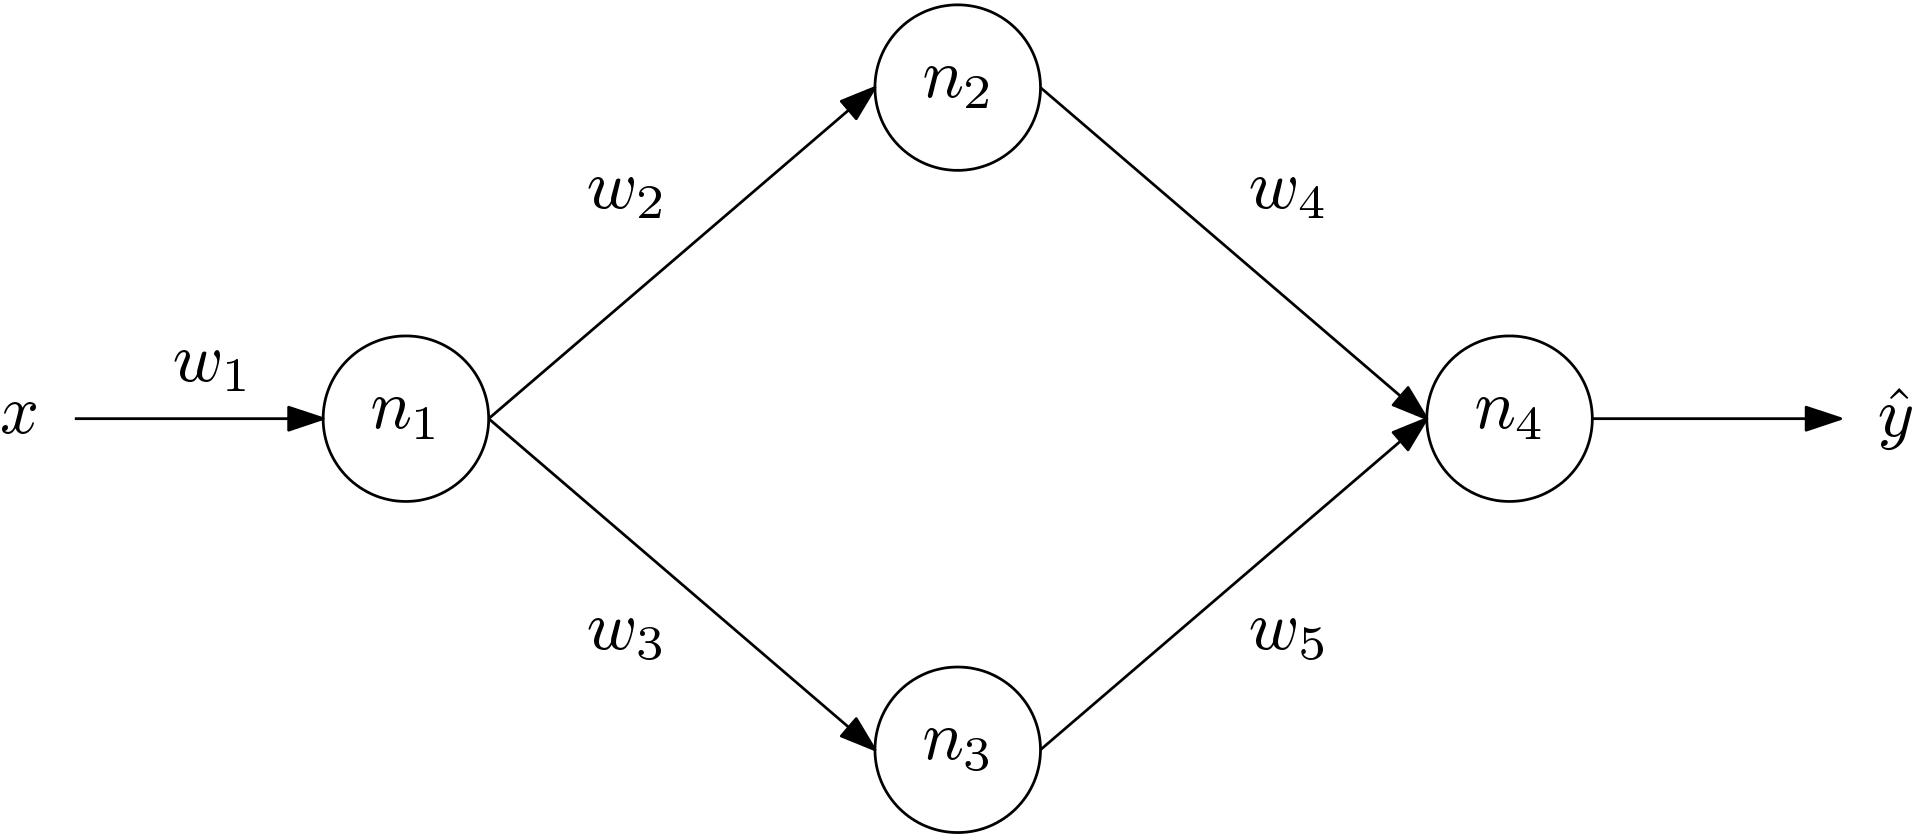
\includegraphics{images/a4_network.png}
\caption{Figure 1}
\end{figure}

It has single input \(x\), and three layers with respectively one, two,
and one neurons. The activation function of the neurons is ReLU.

The parameters \(w_1\), \(w_2\), \(w_3\), \(w_4\), and \(w_5\) (no
biases) are initialized to the following values \(w_1 = 2, w_2 = 1\),
\(w_3 = 2\), \(w_4 = 4\), and \(w_5 = 1\). Implement a single update
step of the gradient descent algorithm by hand. Run the update state for
the data point \((x=2, y=3)\):

The goal is to model the relationship between two continuous variables.
The learning rate is set to \(0.1\)

Provide the solution in the following format:

\begin{itemize}
\tightlist
\item
  A choice for a loss function
\item
  Compute graph for training the neural network
\item
  Partial derivative expression for each of the parameters in the model
\item
  The update expression for each of the parameters for each of the
  data-points
\item
  The final value of all five parameters after the single step in the
  gradient descent algorithm
\end{itemize}

The Python code for simple computational graph nodes, as seen in the
tutorial session, is provided in the cell below (run the cell to load
the code, and again to run the code). Extend the nodes so they can be
used to implement the network described above. Implement the network
with the same initial weights and the correct learning rate, and verify
your hand-made calculations. Add comments to your code or provide a
separate description to explain the changes you have made.

    \begin{Verbatim}[commandchars=\\\{\}]
{\color{incolor}In [{\color{incolor}3}]:} \PY{c+c1}{\PYZsh{} \PYZpc{}load basic\PYZus{}graph.py}
        \PY{l+s+sd}{\PYZsq{}\PYZsq{}\PYZsq{}}
        \PY{l+s+sd}{Implementations of nodes for a computation graph. Each node}
        \PY{l+s+sd}{has a forward pass and a backward pass function, allowing}
        \PY{l+s+sd}{for the evaluation and backpropagation of data.}
        \PY{l+s+sd}{\PYZsq{}\PYZsq{}\PYZsq{}}
        
        \PY{k+kn}{from} \PY{n+nn}{abc} \PY{k}{import} \PY{n}{ABC}\PY{p}{,} \PY{n}{abstractmethod}
        \PY{k+kn}{import} \PY{n+nn}{math}
        \PY{k+kn}{import} \PY{n+nn}{time}
        
        
        \PY{k}{class} \PY{n+nc}{Node}\PY{p}{(}\PY{n+nb}{object}\PY{p}{)}\PY{p}{:}
        
            \PY{k}{def} \PY{n+nf}{\PYZus{}\PYZus{}init\PYZus{}\PYZus{}}\PY{p}{(}\PY{n+nb+bp}{self}\PY{p}{,} \PY{n}{inputs}\PY{p}{)}\PY{p}{:}
                \PY{n+nb+bp}{self}\PY{o}{.}\PY{n}{inputs} \PY{o}{=} \PY{n}{inputs}
        
            \PY{n+nd}{@abstractmethod}
            \PY{k}{def} \PY{n+nf}{forward}\PY{p}{(}\PY{n+nb+bp}{self}\PY{p}{)}\PY{p}{:}
                \PY{l+s+sd}{\PYZsq{}\PYZsq{}\PYZsq{} Feed\PYZhy{}forward the result \PYZsq{}\PYZsq{}\PYZsq{}}
                \PY{k}{raise} \PY{n+ne}{NotImplementedError}\PY{p}{(}\PY{l+s+s2}{\PYZdq{}}\PY{l+s+s2}{Missing forward\PYZhy{}propagation method.}\PY{l+s+s2}{\PYZdq{}}\PY{p}{)}
        
            \PY{n+nd}{@abstractmethod}
            \PY{k}{def} \PY{n+nf}{backward}\PY{p}{(}\PY{n+nb+bp}{self}\PY{p}{,} \PY{n}{d}\PY{p}{)}\PY{p}{:}
                \PY{l+s+sd}{\PYZsq{}\PYZsq{}\PYZsq{} Back\PYZhy{}propagate the error}
        \PY{l+s+sd}{            d is the delta of the subsequent node in the network \PYZsq{}\PYZsq{}\PYZsq{}}
                \PY{k}{raise} \PY{n+ne}{NotImplementedError}\PY{p}{(}\PY{l+s+s2}{\PYZdq{}}\PY{l+s+s2}{Missing back\PYZhy{}propagation method.}\PY{l+s+s2}{\PYZdq{}}\PY{p}{)}
        
        
        \PY{k}{class} \PY{n+nc}{ConstantNode}\PY{p}{(}\PY{n}{Node}\PY{p}{)}\PY{p}{:}
        
            \PY{k}{def} \PY{n+nf}{\PYZus{}\PYZus{}init\PYZus{}\PYZus{}}\PY{p}{(}\PY{n+nb+bp}{self}\PY{p}{,} \PY{n}{value}\PY{p}{)}\PY{p}{:}
                \PY{n+nb+bp}{self}\PY{o}{.}\PY{n}{output} \PY{o}{=} \PY{n}{value}
        
            \PY{k}{def} \PY{n+nf}{forward}\PY{p}{(}\PY{n+nb+bp}{self}\PY{p}{)}\PY{p}{:}
                \PY{k}{return} \PY{n+nb+bp}{self}\PY{o}{.}\PY{n}{output}
        
            \PY{k}{def} \PY{n+nf}{backward}\PY{p}{(}\PY{n+nb+bp}{self}\PY{p}{,} \PY{n}{d}\PY{p}{)}\PY{p}{:}
                \PY{k}{pass}
        
        
        \PY{k}{class} \PY{n+nc}{VariableNode}\PY{p}{(}\PY{n}{Node}\PY{p}{)}\PY{p}{:}
        
            \PY{k}{def} \PY{n+nf}{\PYZus{}\PYZus{}init\PYZus{}\PYZus{}}\PY{p}{(}\PY{n+nb+bp}{self}\PY{p}{,} \PY{n}{value}\PY{p}{)}\PY{p}{:}
                \PY{n+nb+bp}{self}\PY{o}{.}\PY{n}{output} \PY{o}{=} \PY{n}{value}
        
            \PY{k}{def} \PY{n+nf}{forward}\PY{p}{(}\PY{n+nb+bp}{self}\PY{p}{)}\PY{p}{:}
                \PY{k}{return} \PY{n+nb+bp}{self}\PY{o}{.}\PY{n}{output}
        
            \PY{k}{def} \PY{n+nf}{backward}\PY{p}{(}\PY{n+nb+bp}{self}\PY{p}{,} \PY{n}{d}\PY{p}{)}\PY{p}{:}
                \PY{n+nb+bp}{self}\PY{o}{.}\PY{n}{output} \PY{o}{\PYZhy{}}\PY{o}{=} \PY{l+m+mf}{0.1} \PY{o}{*} \PY{n}{d} \PY{c+c1}{\PYZsh{} Gradient Descent}
        
        
        \PY{k}{class} \PY{n+nc}{AdditionNode}\PY{p}{(}\PY{n}{Node}\PY{p}{)}\PY{p}{:}
        
            \PY{k}{def} \PY{n+nf}{forward}\PY{p}{(}\PY{n+nb+bp}{self}\PY{p}{)}\PY{p}{:}
                \PY{n+nb+bp}{self}\PY{o}{.}\PY{n}{output} \PY{o}{=} \PY{n+nb}{sum}\PY{p}{(}\PY{p}{[}\PY{n}{i}\PY{o}{.}\PY{n}{forward}\PY{p}{(}\PY{p}{)} \PY{k}{for} \PY{n}{i} \PY{o+ow}{in} \PY{n+nb+bp}{self}\PY{o}{.}\PY{n}{inputs}\PY{p}{]}\PY{p}{)}
                \PY{k}{return} \PY{n+nb+bp}{self}\PY{o}{.}\PY{n}{output}
        
            \PY{k}{def} \PY{n+nf}{backward}\PY{p}{(}\PY{n+nb+bp}{self}\PY{p}{,} \PY{n}{d}\PY{p}{)}\PY{p}{:}
                \PY{k}{for} \PY{n}{i} \PY{o+ow}{in} \PY{n+nb+bp}{self}\PY{o}{.}\PY{n}{inputs}\PY{p}{:}
                    \PY{n}{i}\PY{o}{.}\PY{n}{backward}\PY{p}{(}\PY{n}{d}\PY{p}{)}
        
        
        \PY{k}{class} \PY{n+nc}{MultiplicationNode}\PY{p}{(}\PY{n}{Node}\PY{p}{)}\PY{p}{:}
        
            \PY{k}{def} \PY{n+nf}{forward}\PY{p}{(}\PY{n+nb+bp}{self}\PY{p}{)}\PY{p}{:}
                \PY{n+nb+bp}{self}\PY{o}{.}\PY{n}{output} \PY{o}{=} \PY{n+nb+bp}{self}\PY{o}{.}\PY{n}{inputs}\PY{p}{[}\PY{l+m+mi}{0}\PY{p}{]}\PY{o}{.}\PY{n}{forward}\PY{p}{(}\PY{p}{)} \PY{o}{*} \PY{n+nb+bp}{self}\PY{o}{.}\PY{n}{inputs}\PY{p}{[}\PY{l+m+mi}{1}\PY{p}{]}\PY{o}{.}\PY{n}{forward}\PY{p}{(}\PY{p}{)}
                \PY{k}{return} \PY{n+nb+bp}{self}\PY{o}{.}\PY{n}{output}
        
            \PY{k}{def} \PY{n+nf}{backward}\PY{p}{(}\PY{n+nb+bp}{self}\PY{p}{,} \PY{n}{d}\PY{p}{)}\PY{p}{:}
                \PY{n+nb+bp}{self}\PY{o}{.}\PY{n}{inputs}\PY{p}{[}\PY{l+m+mi}{0}\PY{p}{]}\PY{o}{.}\PY{n}{backward}\PY{p}{(}\PY{n}{d} \PY{o}{*} \PY{n+nb+bp}{self}\PY{o}{.}\PY{n}{inputs}\PY{p}{[}\PY{l+m+mi}{1}\PY{p}{]}\PY{o}{.}\PY{n}{output}\PY{p}{)}
                \PY{n+nb+bp}{self}\PY{o}{.}\PY{n}{inputs}\PY{p}{[}\PY{l+m+mi}{1}\PY{p}{]}\PY{o}{.}\PY{n}{backward}\PY{p}{(}\PY{n}{d} \PY{o}{*} \PY{n+nb+bp}{self}\PY{o}{.}\PY{n}{inputs}\PY{p}{[}\PY{l+m+mi}{0}\PY{p}{]}\PY{o}{.}\PY{n}{output}\PY{p}{)}
        
        
        \PY{k}{class} \PY{n+nc}{MSENode}\PY{p}{(}\PY{n}{Node}\PY{p}{)}\PY{p}{:}
        
            \PY{k}{def} \PY{n+nf}{forward}\PY{p}{(}\PY{n+nb+bp}{self}\PY{p}{)}\PY{p}{:}
                \PY{n+nb+bp}{self}\PY{o}{.}\PY{n}{output} \PY{o}{=} \PY{l+m+mf}{0.5} \PY{o}{*} \PY{p}{(}
                    \PY{n+nb+bp}{self}\PY{o}{.}\PY{n}{inputs}\PY{p}{[}\PY{l+m+mi}{0}\PY{p}{]}\PY{o}{.}\PY{n}{forward}\PY{p}{(}\PY{p}{)} \PY{o}{\PYZhy{}} \PY{n+nb+bp}{self}\PY{o}{.}\PY{n}{inputs}\PY{p}{[}\PY{l+m+mi}{1}\PY{p}{]}\PY{o}{.}\PY{n}{forward}\PY{p}{(}\PY{p}{)}\PY{p}{)}\PY{o}{*}\PY{o}{*}\PY{l+m+mi}{2}
                \PY{k}{return} \PY{n+nb+bp}{self}\PY{o}{.}\PY{n}{output}
        
            \PY{k}{def} \PY{n+nf}{backward}\PY{p}{(}\PY{n+nb+bp}{self}\PY{p}{,} \PY{n}{d}\PY{p}{)}\PY{p}{:}
                \PY{n+nb+bp}{self}\PY{o}{.}\PY{n}{inputs}\PY{p}{[}\PY{l+m+mi}{0}\PY{p}{]}\PY{o}{.}\PY{n}{backward}\PY{p}{(}\PY{n}{d} \PY{o}{*} \PY{p}{(}\PY{n+nb+bp}{self}\PY{o}{.}\PY{n}{inputs}\PY{p}{[}\PY{l+m+mi}{0}\PY{p}{]}\PY{o}{.}\PY{n}{output} \PY{o}{\PYZhy{}} \PY{n+nb+bp}{self}\PY{o}{.}\PY{n}{inputs}\PY{p}{[}\PY{l+m+mi}{1}\PY{p}{]}\PY{o}{.}\PY{n}{output}\PY{p}{)}\PY{p}{)}
                \PY{n+nb+bp}{self}\PY{o}{.}\PY{n}{inputs}\PY{p}{[}\PY{l+m+mi}{1}\PY{p}{]}\PY{o}{.}\PY{n}{backward}\PY{p}{(}\PY{n}{d} \PY{o}{*} \PY{p}{(}\PY{n+nb+bp}{self}\PY{o}{.}\PY{n}{inputs}\PY{p}{[}\PY{l+m+mi}{1}\PY{p}{]}\PY{o}{.}\PY{n}{output} \PY{o}{\PYZhy{}} \PY{n+nb+bp}{self}\PY{o}{.}\PY{n}{inputs}\PY{p}{[}\PY{l+m+mi}{0}\PY{p}{]}\PY{o}{.}\PY{n}{output}\PY{p}{)}\PY{p}{)}
        
        
        \PY{k}{class} \PY{n+nc}{SigmoidNode}\PY{p}{(}\PY{n}{Node}\PY{p}{)}\PY{p}{:}
        
            \PY{k}{def} \PY{n+nf}{forward}\PY{p}{(}\PY{n+nb+bp}{self}\PY{p}{)}\PY{p}{:}
                \PY{n+nb+bp}{self}\PY{o}{.}\PY{n}{output} \PY{o}{=} \PY{l+m+mf}{1.0} \PY{o}{/} \PY{p}{(}\PY{l+m+mf}{1.0} \PY{o}{+} \PY{n}{math}\PY{o}{.}\PY{n}{exp}\PY{p}{(}\PY{o}{\PYZhy{}}\PY{n+nb+bp}{self}\PY{o}{.}\PY{n}{inputs}\PY{p}{[}\PY{l+m+mi}{0}\PY{p}{]}\PY{o}{.}\PY{n}{forward}\PY{p}{(}\PY{p}{)}\PY{p}{)}\PY{p}{)}
                \PY{k}{return} \PY{n+nb+bp}{self}\PY{o}{.}\PY{n}{output}
        
            \PY{k}{def} \PY{n+nf}{backward}\PY{p}{(}\PY{n+nb+bp}{self}\PY{p}{,} \PY{n}{d}\PY{p}{)}\PY{p}{:}
                \PY{n+nb+bp}{self}\PY{o}{.}\PY{n}{inputs}\PY{p}{[}\PY{l+m+mi}{0}\PY{p}{]}\PY{o}{.}\PY{n}{backward}\PY{p}{(}\PY{n}{d} \PY{o}{*} \PY{n+nb+bp}{self}\PY{o}{.}\PY{n}{output} \PY{o}{*} \PY{p}{(}\PY{l+m+mf}{1.0} \PY{o}{\PYZhy{}} \PY{n+nb+bp}{self}\PY{o}{.}\PY{n}{output}\PY{p}{)}\PY{p}{)}
        
        \PY{k}{class} \PY{n+nc}{ReLUNode}\PY{p}{(}\PY{n+nb}{object}\PY{p}{)}\PY{p}{:}
        
            \PY{k}{def} \PY{n+nf}{forward}\PY{p}{(}\PY{n+nb+bp}{self}\PY{p}{)}\PY{p}{:}
                \PY{k}{raise} \PY{n+ne}{NotImplementedError}\PY{p}{(}\PY{l+s+s2}{\PYZdq{}}\PY{l+s+s2}{Forward pass for ReLU activation node has not been implemented yet.}\PY{l+s+s2}{\PYZdq{}}\PY{p}{)}
        
            \PY{k}{def} \PY{n+nf}{backward}\PY{p}{(}\PY{n+nb+bp}{self}\PY{p}{,} \PY{n}{d}\PY{p}{)}\PY{p}{:}
                \PY{k}{raise} \PY{n+ne}{NotImplementedError}\PY{p}{(}\PY{l+s+s2}{\PYZdq{}}\PY{l+s+s2}{Backward pass for ReLU activation node has not been implemented yet.}\PY{l+s+s2}{\PYZdq{}}\PY{p}{)}
        
        \PY{k}{class} \PY{n+nc}{TanhNode}\PY{p}{(}\PY{n+nb}{object}\PY{p}{)}\PY{p}{:}
        
            \PY{k}{def} \PY{n+nf}{forward}\PY{p}{(}\PY{n+nb+bp}{self}\PY{p}{)}\PY{p}{:}
                \PY{k}{raise} \PY{n+ne}{NotImplementedError}\PY{p}{(}\PY{l+s+s2}{\PYZdq{}}\PY{l+s+s2}{Forward pass for tanh activation node has not been implemented yet.}\PY{l+s+s2}{\PYZdq{}}\PY{p}{)}
        
            \PY{k}{def} \PY{n+nf}{backward}\PY{p}{(}\PY{n+nb+bp}{self}\PY{p}{,} \PY{n}{d}\PY{p}{)}\PY{p}{:}
                \PY{k}{raise} \PY{n+ne}{NotImplementedError}\PY{p}{(}\PY{l+s+s2}{\PYZdq{}}\PY{l+s+s2}{Backward pass for tanh activation node has not been implemented yet.}\PY{l+s+s2}{\PYZdq{}}\PY{p}{)}
        
        \PY{c+c1}{\PYZsh{} Example graph as shown in MLP lecture slides}
        \PY{k}{class} \PY{n+nc}{SampleGraph}\PY{p}{(}\PY{n+nb}{object}\PY{p}{)}\PY{p}{:}
        
            \PY{k}{def} \PY{n+nf}{\PYZus{}\PYZus{}init\PYZus{}\PYZus{}}\PY{p}{(}\PY{n+nb+bp}{self}\PY{p}{,} \PY{n}{x}\PY{p}{,} \PY{n}{y}\PY{p}{,} \PY{n}{w}\PY{p}{,} \PY{n}{b}\PY{p}{)}\PY{p}{:}
                \PY{l+s+sd}{\PYZsq{}\PYZsq{}\PYZsq{} x: input}
        \PY{l+s+sd}{            y: expected output}
        \PY{l+s+sd}{            w: initial weight}
        \PY{l+s+sd}{            b: initial bias \PYZsq{}\PYZsq{}\PYZsq{}}
                \PY{n+nb+bp}{self}\PY{o}{.}\PY{n}{w} \PY{o}{=} \PY{n}{VariableNode}\PY{p}{(}\PY{n}{w}\PY{p}{)}
                \PY{n+nb+bp}{self}\PY{o}{.}\PY{n}{b} \PY{o}{=} \PY{n}{VariableNode}\PY{p}{(}\PY{n}{b}\PY{p}{)}
                \PY{n+nb+bp}{self}\PY{o}{.}\PY{n}{graph} \PY{o}{=} \PY{n}{MSENode}\PY{p}{(}\PY{p}{[}
                    \PY{n}{AdditionNode}\PY{p}{(}\PY{p}{[}
                        \PY{n}{MultiplicationNode}\PY{p}{(}\PY{p}{[}
                            \PY{n}{ConstantNode}\PY{p}{(}\PY{n}{x}\PY{p}{)}\PY{p}{,}
                            \PY{n+nb+bp}{self}\PY{o}{.}\PY{n}{w}
                        \PY{p}{]}\PY{p}{)}\PY{p}{,}
                        \PY{n}{MultiplicationNode}\PY{p}{(}\PY{p}{[}
                            \PY{n+nb+bp}{self}\PY{o}{.}\PY{n}{b}\PY{p}{,}
                            \PY{n}{ConstantNode}\PY{p}{(}\PY{l+m+mi}{1}\PY{p}{)}
                        \PY{p}{]}\PY{p}{)}
                    \PY{p}{]}\PY{p}{)}\PY{p}{,}
                    \PY{n}{ConstantNode}\PY{p}{(}\PY{n}{y}\PY{p}{)}
                \PY{p}{]}\PY{p}{)}
        
            \PY{k}{def} \PY{n+nf}{forward}\PY{p}{(}\PY{n+nb+bp}{self}\PY{p}{)}\PY{p}{:}
                \PY{k}{return} \PY{n+nb+bp}{self}\PY{o}{.}\PY{n}{graph}\PY{o}{.}\PY{n}{forward}\PY{p}{(}\PY{p}{)}
        
            \PY{k}{def} \PY{n+nf}{backward}\PY{p}{(}\PY{n+nb+bp}{self}\PY{p}{,} \PY{n}{d}\PY{p}{)}\PY{p}{:}
                \PY{n+nb+bp}{self}\PY{o}{.}\PY{n}{graph}\PY{o}{.}\PY{n}{backward}\PY{p}{(}\PY{n}{d}\PY{p}{)}
        
        
        \PY{k}{class} \PY{n+nc}{Neuron}\PY{p}{(}\PY{n}{Node}\PY{p}{)}\PY{p}{:}
        
            \PY{k}{def} \PY{n+nf}{\PYZus{}\PYZus{}init\PYZus{}\PYZus{}}\PY{p}{(}\PY{n+nb+bp}{self}\PY{p}{,} \PY{n}{inputs}\PY{p}{,} \PY{n}{weights}\PY{p}{,} \PY{n}{activation}\PY{p}{)}\PY{p}{:}
                \PY{l+s+sd}{\PYZsq{}\PYZsq{}\PYZsq{} weights: list of initial weights, same length as inputs \PYZsq{}\PYZsq{}\PYZsq{}}
                \PY{n+nb+bp}{self}\PY{o}{.}\PY{n}{inputs} \PY{o}{=} \PY{n}{inputs}
                \PY{c+c1}{\PYZsh{} Initialize a weight for each input}
                \PY{n+nb+bp}{self}\PY{o}{.}\PY{n}{weights} \PY{o}{=} \PY{p}{[}\PY{n}{VariableNode}\PY{p}{(}\PY{n}{weight}\PY{p}{)} \PY{k}{for} \PY{n}{weight} \PY{o+ow}{in} \PY{n}{weights}\PY{p}{]}
                \PY{c+c1}{\PYZsh{} Neurons normally have a bias, ignore for this assignment}
                \PY{c+c1}{\PYZsh{}self.bias = VariableNode(bias, \PYZdq{}b\PYZdq{})}
        
                \PY{c+c1}{\PYZsh{} Multiplication node for each pair of inputs and weights}
                \PY{n}{mults} \PY{o}{=} \PY{p}{[}\PY{n}{MultiplicationNode}\PY{p}{(}\PY{p}{[}\PY{n}{i}\PY{p}{,} \PY{n}{w}\PY{p}{]}\PY{p}{)} \PY{k}{for} \PY{n}{i}\PY{p}{,} \PY{n}{w}\PY{p}{,} \PY{o+ow}{in} \PY{n+nb}{zip}\PY{p}{(}\PY{n+nb+bp}{self}\PY{o}{.}\PY{n}{inputs}\PY{p}{,} \PY{n+nb+bp}{self}\PY{o}{.}\PY{n}{weights}\PY{p}{)}\PY{p}{]}
                \PY{c+c1}{\PYZsh{} Neurons normally have a bias, ignore for this assignment}
                \PY{c+c1}{\PYZsh{}mults.append(MultiplicationNode([self.bias, ConstantNode(1)]))}
        
                \PY{c+c1}{\PYZsh{} Sum all multiplication results}
                \PY{n}{added} \PY{o}{=} \PY{n}{AdditionNode}\PY{p}{(}\PY{n}{mults}\PY{p}{)}
        
                \PY{c+c1}{\PYZsh{} Apply activation function}
                \PY{k}{if} \PY{n}{activation} \PY{o}{==} \PY{l+s+s1}{\PYZsq{}}\PY{l+s+s1}{sigmoid}\PY{l+s+s1}{\PYZsq{}}\PY{p}{:}
                    \PY{n+nb+bp}{self}\PY{o}{.}\PY{n}{graph} \PY{o}{=} \PY{n}{SigmoidNode}\PY{p}{(}\PY{p}{[}\PY{n}{added}\PY{p}{]}\PY{p}{)}
                \PY{k}{elif} \PY{n}{activation} \PY{o}{==} \PY{l+s+s1}{\PYZsq{}}\PY{l+s+s1}{relu}\PY{l+s+s1}{\PYZsq{}}\PY{p}{:}
                    \PY{n+nb+bp}{self}\PY{o}{.}\PY{n}{graph} \PY{o}{=} \PY{n}{ReLUNode}\PY{p}{(}\PY{p}{[}\PY{n}{added}\PY{p}{]}\PY{p}{)}
                \PY{k}{elif} \PY{n}{activation} \PY{o}{==} \PY{l+s+s1}{\PYZsq{}}\PY{l+s+s1}{tanh}\PY{l+s+s1}{\PYZsq{}}\PY{p}{:}
                    \PY{n+nb+bp}{self}\PY{o}{.}\PY{n}{graph} \PY{o}{=} \PY{n}{TanhNode}\PY{p}{(}\PY{p}{[}\PY{n}{added}\PY{p}{]}\PY{p}{)}
                \PY{k}{else}\PY{p}{:}
                    \PY{k}{raise} \PY{n+ne}{ValueError}\PY{p}{(}\PY{l+s+s2}{\PYZdq{}}\PY{l+s+s2}{Unknown activation function.}\PY{l+s+s2}{\PYZdq{}}\PY{p}{)}
        
            \PY{k}{def} \PY{n+nf}{forward}\PY{p}{(}\PY{n+nb+bp}{self}\PY{p}{)}\PY{p}{:}
                \PY{k}{return} \PY{n+nb+bp}{self}\PY{o}{.}\PY{n}{graph}\PY{o}{.}\PY{n}{forward}\PY{p}{(}\PY{p}{)}
        
            \PY{k}{def} \PY{n+nf}{backward}\PY{p}{(}\PY{n+nb+bp}{self}\PY{p}{,} \PY{n}{d}\PY{p}{)}\PY{p}{:}
                \PY{n+nb+bp}{self}\PY{o}{.}\PY{n}{graph}\PY{o}{.}\PY{n}{backward}\PY{p}{(}\PY{n}{d}\PY{p}{)}
        
            \PY{k}{def} \PY{n+nf}{set\PYZus{}weights}\PY{p}{(}\PY{n+nb+bp}{self}\PY{p}{,} \PY{n}{new\PYZus{}weights}\PY{p}{)}\PY{p}{:}
                \PY{k}{for} \PY{n}{i} \PY{o+ow}{in} \PY{n+nb}{len}\PY{p}{(}\PY{n}{new\PYZus{}weights}\PY{p}{)}\PY{p}{:}
                    \PY{n+nb+bp}{self}\PY{o}{.}\PY{n}{weights}\PY{p}{[}\PY{n}{i}\PY{p}{]}\PY{o}{.}\PY{n}{output} \PY{o}{=} \PY{n}{new\PYZus{}weights}\PY{p}{[}\PY{n}{i}\PY{p}{]}
        
            \PY{k}{def} \PY{n+nf}{get\PYZus{}weights}\PY{p}{(}\PY{n+nb+bp}{self}\PY{p}{)}\PY{p}{:}
                \PY{k}{return} \PY{p}{[}\PY{n}{weight}\PY{o}{.}\PY{n}{output} \PY{k}{for} \PY{n}{weight} \PY{o+ow}{in} \PY{n+nb+bp}{self}\PY{o}{.}\PY{n}{weights}\PY{p}{]}
        
        \PY{k}{if} \PY{n+nv+vm}{\PYZus{}\PYZus{}name\PYZus{}\PYZus{}} \PY{o}{==} \PY{l+s+s1}{\PYZsq{}}\PY{l+s+s1}{\PYZus{}\PYZus{}main\PYZus{}\PYZus{}}\PY{l+s+s1}{\PYZsq{}}\PY{p}{:}
            \PY{n+nb}{print}\PY{p}{(}\PY{l+s+s2}{\PYZdq{}}\PY{l+s+s2}{Loaded simple graph nodes}\PY{l+s+s2}{\PYZdq{}}\PY{p}{)}
        
            \PY{c+c1}{\PYZsh{} Example network}
            \PY{c+c1}{\PYZsh{}sg = SampleGraph(2, 2, 2, 1)}
            \PY{c+c1}{\PYZsh{}prediction = sg.forward()}
            \PY{c+c1}{\PYZsh{}print(\PYZdq{}Initial prediction is\PYZdq{}, prediction)}
            \PY{c+c1}{\PYZsh{}sg.backward(1)}
            \PY{c+c1}{\PYZsh{}print(\PYZdq{}w has new value\PYZdq{}, sg.w.output)}
            \PY{c+c1}{\PYZsh{}print(\PYZdq{}b has new value\PYZdq{}, sg.b.output)}
        
            \PY{c+c1}{\PYZsh{} Run your network here}
        \PY{k}{class} \PY{n+nc}{MyGraph}\PY{p}{(}\PY{n+nb}{object}\PY{p}{)}\PY{p}{:}
        
            \PY{k}{def} \PY{n+nf}{\PYZus{}\PYZus{}init\PYZus{}\PYZus{}}\PY{p}{(}\PY{n+nb+bp}{self}\PY{p}{,} \PY{n}{x}\PY{p}{,} \PY{n}{y}\PY{p}{,} \PY{n}{weigths}\PY{p}{)}\PY{p}{:}
                \PY{l+s+sd}{\PYZsq{}\PYZsq{}\PYZsq{} x: input}
        \PY{l+s+sd}{            y: expected output}
        \PY{l+s+sd}{            w: initial weight}
        \PY{l+s+sd}{            b: initial bias \PYZsq{}\PYZsq{}\PYZsq{}}
                               
                \PY{n+nb+bp}{self}\PY{o}{.}\PY{n}{weights} \PY{o}{=} \PY{p}{[}\PY{n}{VariableNode}\PY{p}{(}\PY{n}{weight}\PY{p}{)} \PY{k}{for} \PY{n}{weight} \PY{o+ow}{in} \PY{n}{weigths}\PY{p}{]}
                
                \PY{n+nb+bp}{self}\PY{o}{.}\PY{n}{z1} \PY{o}{=} \PY{n}{MultiplicationNode}\PY{p}{(}\PY{p}{[}\PY{n}{ConstantNode}\PY{p}{(}\PY{n}{x}\PY{p}{)}\PY{p}{,}\PY{n+nb+bp}{self}\PY{o}{.}\PY{n}{weights}\PY{p}{[}\PY{l+m+mi}{0}\PY{p}{]}\PY{p}{]}\PY{p}{)}
                \PY{n+nb+bp}{self}\PY{o}{.}\PY{n}{n1} \PY{o}{=} \PY{n}{SigmoidNode}\PY{p}{(}\PY{p}{[}\PY{n+nb+bp}{self}\PY{o}{.}\PY{n}{z1}\PY{p}{]}\PY{p}{)}
                \PY{n+nb+bp}{self}\PY{o}{.}\PY{n}{z2} \PY{o}{=} \PY{n}{MultiplicationNode}\PY{p}{(}\PY{p}{[}\PY{n+nb+bp}{self}\PY{o}{.}\PY{n}{n1}\PY{p}{,} \PY{n+nb+bp}{self}\PY{o}{.}\PY{n}{weights}\PY{p}{[}\PY{l+m+mi}{1}\PY{p}{]}\PY{p}{]}\PY{p}{)}
                \PY{n+nb+bp}{self}\PY{o}{.}\PY{n}{n2} \PY{o}{=} \PY{n}{SigmoidNode}\PY{p}{(}\PY{p}{[}\PY{n+nb+bp}{self}\PY{o}{.}\PY{n}{z2}\PY{p}{]}\PY{p}{)}
                \PY{n+nb+bp}{self}\PY{o}{.}\PY{n}{z3} \PY{o}{=} \PY{n}{MultiplicationNode}\PY{p}{(}\PY{p}{[}\PY{n+nb+bp}{self}\PY{o}{.}\PY{n}{n1}\PY{p}{,} \PY{n+nb+bp}{self}\PY{o}{.}\PY{n}{weights}\PY{p}{[}\PY{l+m+mi}{2}\PY{p}{]}\PY{p}{]}\PY{p}{)}
                \PY{n+nb+bp}{self}\PY{o}{.}\PY{n}{n3} \PY{o}{=} \PY{n}{SigmoidNode}\PY{p}{(}\PY{p}{[}\PY{n+nb+bp}{self}\PY{o}{.}\PY{n}{z3}\PY{p}{]}\PY{p}{)}
                \PY{n+nb+bp}{self}\PY{o}{.}\PY{n}{z4} \PY{o}{=} \PY{n}{AdditionNode}\PY{p}{(}\PY{p}{[}\PY{n}{MultiplicationNode}\PY{p}{(}\PY{p}{[}
                                     \PY{n+nb+bp}{self}\PY{o}{.}\PY{n}{n2}\PY{p}{,}
                                     \PY{n+nb+bp}{self}\PY{o}{.}\PY{n}{weights}\PY{p}{[}\PY{l+m+mi}{3}\PY{p}{]}\PY{p}{]}\PY{p}{)}\PY{p}{,}
                                     \PY{n}{MultiplicationNode}\PY{p}{(}\PY{p}{[}
                                     \PY{n+nb+bp}{self}\PY{o}{.}\PY{n}{n3}\PY{p}{,}
                                     \PY{n+nb+bp}{self}\PY{o}{.}\PY{n}{weights}\PY{p}{[}\PY{l+m+mi}{4}\PY{p}{]}\PY{p}{]}\PY{p}{)}\PY{p}{]}\PY{p}{)}
                \PY{n+nb+bp}{self}\PY{o}{.}\PY{n}{n4} \PY{o}{=} \PY{n}{SigmoidNode}\PY{p}{(}\PY{p}{[}\PY{n+nb+bp}{self}\PY{o}{.}\PY{n}{z4}\PY{p}{]}\PY{p}{)}
                \PY{n+nb+bp}{self}\PY{o}{.}\PY{n}{graph} \PY{o}{=} \PY{n}{MSENode}\PY{p}{(}\PY{p}{[}\PY{n+nb+bp}{self}\PY{o}{.}\PY{n}{n4}\PY{p}{,}\PY{n}{ConstantNode}\PY{p}{(}\PY{n}{y}\PY{p}{)}\PY{p}{]}\PY{p}{)}
        
            \PY{k}{def} \PY{n+nf}{forward}\PY{p}{(}\PY{n+nb+bp}{self}\PY{p}{)}\PY{p}{:}
                \PY{k}{return} \PY{n+nb+bp}{self}\PY{o}{.}\PY{n}{graph}\PY{o}{.}\PY{n}{forward}\PY{p}{(}\PY{p}{)}
        
            \PY{k}{def} \PY{n+nf}{backward}\PY{p}{(}\PY{n+nb+bp}{self}\PY{p}{,} \PY{n}{d}\PY{p}{)}\PY{p}{:}
                \PY{n+nb+bp}{self}\PY{o}{.}\PY{n}{graph}\PY{o}{.}\PY{n}{backward}\PY{p}{(}\PY{n}{d}\PY{p}{)}
            \PY{k}{def} \PY{n+nf}{set\PYZus{}weights}\PY{p}{(}\PY{n+nb+bp}{self}\PY{p}{,} \PY{n}{new\PYZus{}weights}\PY{p}{)}\PY{p}{:}
                \PY{k}{for} \PY{n}{i} \PY{o+ow}{in} \PY{n+nb}{len}\PY{p}{(}\PY{n}{new\PYZus{}weights}\PY{p}{)}\PY{p}{:}
                    \PY{n+nb+bp}{self}\PY{o}{.}\PY{n}{weights}\PY{p}{[}\PY{n}{i}\PY{p}{]}\PY{o}{.}\PY{n}{output} \PY{o}{=} \PY{n}{new\PYZus{}weights}\PY{p}{[}\PY{n}{i}\PY{p}{]}
        
            \PY{k}{def} \PY{n+nf}{get\PYZus{}weights}\PY{p}{(}\PY{n+nb+bp}{self}\PY{p}{)}\PY{p}{:}
                \PY{k}{return} \PY{p}{[}\PY{n}{weight}\PY{o}{.}\PY{n}{output} \PY{k}{for} \PY{n}{weight} \PY{o+ow}{in} \PY{n+nb+bp}{self}\PY{o}{.}\PY{n}{weights}\PY{p}{]}
        
        \PY{n}{x}\PY{o}{=}\PY{l+m+mi}{2}
        \PY{n}{y}\PY{o}{=}\PY{l+m+mi}{3}
        \PY{n}{w1}\PY{o}{=}\PY{l+m+mi}{2}
        \PY{n}{w2}\PY{o}{=}\PY{l+m+mi}{1}
        \PY{n}{w3}\PY{o}{=}\PY{l+m+mi}{2}
        \PY{n}{w4}\PY{o}{=}\PY{l+m+mi}{4}
        \PY{n}{w5}\PY{o}{=}\PY{l+m+mi}{1}
        
        
        \PY{n}{sg} \PY{o}{=} \PY{n}{MyGraph}\PY{p}{(}\PY{n}{x}\PY{p}{,} \PY{n}{y}\PY{p}{,}\PY{p}{[}\PY{n}{w1}\PY{p}{,}\PY{n}{w2}\PY{p}{,}\PY{n}{w3}\PY{p}{,}\PY{n}{w4}\PY{p}{,}\PY{n}{w5}\PY{p}{]}\PY{p}{)}
        
        \PY{n}{Error1} \PY{o}{=} \PY{n}{sg}\PY{o}{.}\PY{n}{forward}\PY{p}{(}\PY{p}{)}
        
        \PY{n+nb}{print}\PY{p}{(}\PY{n}{sg}\PY{o}{.}\PY{n}{z1}\PY{o}{.}\PY{n}{output}\PY{p}{)}
        \PY{n+nb}{print}\PY{p}{(}\PY{n}{sg}\PY{o}{.}\PY{n}{n1}\PY{o}{.}\PY{n}{output}\PY{p}{)}
        \PY{n+nb}{print}\PY{p}{(}\PY{n}{sg}\PY{o}{.}\PY{n}{n2}\PY{o}{.}\PY{n}{output}\PY{p}{)}
        \PY{n+nb}{print}\PY{p}{(}\PY{n}{sg}\PY{o}{.}\PY{n}{n3}\PY{o}{.}\PY{n}{output}\PY{p}{)}
        \PY{n+nb}{print}\PY{p}{(}\PY{n}{sg}\PY{o}{.}\PY{n}{n4}\PY{o}{.}\PY{n}{output}\PY{p}{)}
        \PY{n+nb}{print}\PY{p}{(}\PY{l+s+s2}{\PYZdq{}}\PY{l+s+s2}{Graph}\PY{l+s+s2}{\PYZdq{}}\PY{p}{,}\PY{n}{sg}\PY{o}{.}\PY{n}{graph}\PY{o}{.}\PY{n}{output}\PY{p}{)}
        
        \PY{n}{sg}\PY{o}{.}\PY{n}{backward}\PY{p}{(}\PY{n}{sg}\PY{o}{.}\PY{n}{n4}\PY{o}{.}\PY{n}{output}\PY{p}{)}
        
        \PY{n}{new\PYZus{}weights}\PY{o}{=}\PY{n}{sg}\PY{o}{.}\PY{n}{get\PYZus{}weights}\PY{p}{(}\PY{p}{)}
        \PY{n+nb}{print}\PY{p}{(}\PY{l+s+s2}{\PYZdq{}}\PY{l+s+s2}{w has new value}\PY{l+s+s2}{\PYZdq{}}\PY{p}{,} \PY{n}{np}\PY{o}{.}\PY{n}{transpose}\PY{p}{(}\PY{n}{new\PYZus{}weights}\PY{p}{)}\PY{p}{)}
\end{Verbatim}


\begin{Verbatim}[commandchars=\\\{\}]
{\color{outcolor}Out[{\color{outcolor}3}]:} '\textbackslash{}nImplementations of nodes for a computation graph. Each node\textbackslash{}nhas a forward pass and a backward pass function, allowing\textbackslash{}nfor the evaluation and backpropagation of data.\textbackslash{}n'
\end{Verbatim}
            
    \begin{Verbatim}[commandchars=\\\{\}]
Loaded simple graph nodes
4
0.9820137900379085
0.7275076135036415
0.8769681683739503
0.9778387307456168
Graph 2.0445680994362494
w has new value [2.    1.003 2.    4.003 1.004]

    \end{Verbatim}

    \hypertarget{training-deep-models-3-points}{%
\subsection{Training Deep Models (3
points)}\label{training-deep-models-3-points}}

The model in the example code below performs poorly as its depth
increases. Train this model on the MNIST digit detection task.

Examine its training performance by gradually increasing its depth: -
Set the depth to 1 hidden layer - Set the depth to 2 hidden layers - Set
the depth to 3 hidden layers

Modify the model such that you improve its performance when its depth
increases. Train the new model again for the different depths: - Set the
depth to 1 hidden layer - Set the depth to 2 hidden layers - Set the
depth to 3 hidden layers

Submit an explanation for the limitation of the original model. Explain
your modification. Submit your code and 6 plots (can be overlaid) for
the training performance of both models with different depths.

    \begin{Verbatim}[commandchars=\\\{\}]
{\color{incolor}In [{\color{incolor}19}]:} \PY{c+c1}{\PYZsh{} (You don\PYZsq{}t need to change this part of the code)}
         \PY{k+kn}{from} \PY{n+nn}{\PYZus{}\PYZus{}future\PYZus{}\PYZus{}} \PY{k}{import} \PY{n}{print\PYZus{}function}
         \PY{k+kn}{import} \PY{n+nn}{numpy} \PY{k}{as} \PY{n+nn}{np}
         \PY{n}{np}\PY{o}{.}\PY{n}{random}\PY{o}{.}\PY{n}{seed}\PY{p}{(}\PY{l+m+mi}{1234}\PY{p}{)}
         
         \PY{k+kn}{from} \PY{n+nn}{keras}\PY{n+nn}{.}\PY{n+nn}{datasets} \PY{k}{import} \PY{n}{mnist}
         \PY{k+kn}{from} \PY{n+nn}{keras}\PY{n+nn}{.}\PY{n+nn}{models} \PY{k}{import} \PY{n}{Sequential}
         \PY{k+kn}{from} \PY{n+nn}{keras}\PY{n+nn}{.}\PY{n+nn}{layers}\PY{n+nn}{.}\PY{n+nn}{core} \PY{k}{import} \PY{n}{Dense}\PY{p}{,} \PY{n}{Dropout}\PY{p}{,} \PY{n}{Activation}
         \PY{k+kn}{from} \PY{n+nn}{keras}\PY{n+nn}{.}\PY{n+nn}{optimizers} \PY{k}{import} \PY{n}{SGD}
         \PY{k+kn}{from} \PY{n+nn}{keras}\PY{n+nn}{.}\PY{n+nn}{utils} \PY{k}{import} \PY{n}{np\PYZus{}utils}
         \PY{k+kn}{from} \PY{n+nn}{keras}\PY{n+nn}{.}\PY{n+nn}{layers} \PY{k}{import} \PY{n}{Conv2D}\PY{p}{,} \PY{n}{MaxPooling2D}\PY{p}{,} \PY{n}{Conv1D}\PY{p}{,} \PY{n}{Dense}\PY{p}{,} \PY{n}{TimeDistributed}\PY{p}{,} \PY{n}{Activation}
         
         \PY{k+kn}{import} \PY{n+nn}{matplotlib}\PY{n+nn}{.}\PY{n+nn}{pyplot} \PY{k}{as} \PY{n+nn}{plt}
         
         \PY{n}{batch\PYZus{}size} \PY{o}{=} \PY{l+m+mi}{128}
         \PY{n}{nb\PYZus{}classes} \PY{o}{=} \PY{l+m+mi}{10}
         \PY{n}{nb\PYZus{}epoch} \PY{o}{=} \PY{l+m+mi}{10}
\end{Verbatim}


    \begin{Verbatim}[commandchars=\\\{\}]
{\color{incolor}In [{\color{incolor}20}]:} \PY{c+c1}{\PYZsh{} (You don\PYZsq{}t need to change this part of the code)}
         \PY{c+c1}{\PYZsh{} the data, shuffled and split between train and test sets}
         \PY{p}{(}\PY{n}{X\PYZus{}train}\PY{p}{,} \PY{n}{y\PYZus{}train}\PY{p}{)}\PY{p}{,} \PY{p}{(}\PY{n}{X\PYZus{}test}\PY{p}{,} \PY{n}{y\PYZus{}test}\PY{p}{)} \PY{o}{=} \PY{n}{mnist}\PY{o}{.}\PY{n}{load\PYZus{}data}\PY{p}{(}\PY{p}{)}
         
         \PY{n}{X\PYZus{}train} \PY{o}{=} \PY{n}{X\PYZus{}train}\PY{o}{.}\PY{n}{reshape}\PY{p}{(}\PY{l+m+mi}{60000}\PY{p}{,} \PY{l+m+mi}{784}\PY{p}{)}
         \PY{n}{X\PYZus{}test} \PY{o}{=} \PY{n}{X\PYZus{}test}\PY{o}{.}\PY{n}{reshape}\PY{p}{(}\PY{l+m+mi}{10000}\PY{p}{,} \PY{l+m+mi}{784}\PY{p}{)}
         
         \PY{n}{X\PYZus{}train} \PY{o}{=} \PY{n}{X\PYZus{}train}\PY{o}{.}\PY{n}{astype}\PY{p}{(}\PY{l+s+s1}{\PYZsq{}}\PY{l+s+s1}{float32}\PY{l+s+s1}{\PYZsq{}}\PY{p}{)}
         \PY{n}{X\PYZus{}test} \PY{o}{=} \PY{n}{X\PYZus{}test}\PY{o}{.}\PY{n}{astype}\PY{p}{(}\PY{l+s+s1}{\PYZsq{}}\PY{l+s+s1}{float32}\PY{l+s+s1}{\PYZsq{}}\PY{p}{)}
         \PY{n}{X\PYZus{}train} \PY{o}{/}\PY{o}{=} \PY{l+m+mi}{255}
         \PY{n}{X\PYZus{}test} \PY{o}{/}\PY{o}{=} \PY{l+m+mi}{255}
         \PY{n+nb}{print}\PY{p}{(}\PY{n}{X\PYZus{}train}\PY{o}{.}\PY{n}{shape}\PY{p}{[}\PY{l+m+mi}{0}\PY{p}{]}\PY{p}{,} \PY{l+s+s1}{\PYZsq{}}\PY{l+s+s1}{train samples}\PY{l+s+s1}{\PYZsq{}}\PY{p}{)}
         \PY{n+nb}{print}\PY{p}{(}\PY{n}{X\PYZus{}test}\PY{o}{.}\PY{n}{shape}\PY{p}{[}\PY{l+m+mi}{0}\PY{p}{]}\PY{p}{,} \PY{l+s+s1}{\PYZsq{}}\PY{l+s+s1}{test samples}\PY{l+s+s1}{\PYZsq{}}\PY{p}{)}
         
         \PY{c+c1}{\PYZsh{} convert class vectors to binary class matrices}
         \PY{n}{Y\PYZus{}train} \PY{o}{=} \PY{n}{np\PYZus{}utils}\PY{o}{.}\PY{n}{to\PYZus{}categorical}\PY{p}{(}\PY{n}{y\PYZus{}train}\PY{p}{,} \PY{n}{nb\PYZus{}classes}\PY{p}{)}
         \PY{n}{Y\PYZus{}test} \PY{o}{=} \PY{n}{np\PYZus{}utils}\PY{o}{.}\PY{n}{to\PYZus{}categorical}\PY{p}{(}\PY{n}{y\PYZus{}test}\PY{p}{,} \PY{n}{nb\PYZus{}classes}\PY{p}{)}
\end{Verbatim}


    \begin{Verbatim}[commandchars=\\\{\}]
60000 train samples
10000 test samples

    \end{Verbatim}

    \begin{Verbatim}[commandchars=\\\{\}]
{\color{incolor}In [{\color{incolor}21}]:} \PY{c+c1}{\PYZsh{} Use this parameter to change the depth of the model}
\end{Verbatim}


    \begin{Verbatim}[commandchars=\\\{\}]
{\color{incolor}In [{\color{incolor}26}]:} \PY{n}{number\PYZus{}hidden\PYZus{}layers} \PY{o}{=} \PY{l+m+mi}{1}  \PY{c+c1}{\PYZsh{} Number of hidden layers}
         \PY{c+c1}{\PYZsh{} Model}
         \PY{n}{model} \PY{o}{=} \PY{n}{Sequential}\PY{p}{(}\PY{p}{)}
         \PY{n}{model}\PY{o}{.}\PY{n}{add}\PY{p}{(}\PY{n}{Dense}\PY{p}{(}\PY{l+m+mi}{512}\PY{p}{,} \PY{n}{input\PYZus{}shape}\PY{o}{=}\PY{p}{(}\PY{l+m+mi}{784}\PY{p}{,}\PY{p}{)}\PY{p}{,} \PY{n}{activation}\PY{o}{=}\PY{l+s+s1}{\PYZsq{}}\PY{l+s+s1}{sigmoid}\PY{l+s+s1}{\PYZsq{}}\PY{p}{)}\PY{p}{)}
         \PY{n}{model}\PY{o}{.}\PY{n}{add}\PY{p}{(}\PY{n}{Dropout}\PY{p}{(}\PY{l+m+mf}{0.2}\PY{p}{)}\PY{p}{)}
         \PY{k}{while} \PY{n}{number\PYZus{}hidden\PYZus{}layers} \PY{o}{\PYZgt{}} \PY{l+m+mi}{1}\PY{p}{:}
             \PY{n}{model}\PY{o}{.}\PY{n}{add}\PY{p}{(}\PY{n}{Dense}\PY{p}{(}\PY{l+m+mi}{512}\PY{p}{)}\PY{p}{)}
             \PY{n}{model}\PY{o}{.}\PY{n}{add}\PY{p}{(}\PY{n}{Activation}\PY{p}{(}\PY{l+s+s1}{\PYZsq{}}\PY{l+s+s1}{sigmoid}\PY{l+s+s1}{\PYZsq{}}\PY{p}{)}\PY{p}{)}
             \PY{n}{model}\PY{o}{.}\PY{n}{add}\PY{p}{(}\PY{n}{Dropout}\PY{p}{(}\PY{l+m+mf}{0.2}\PY{p}{)}\PY{p}{)}
             \PY{n}{number\PYZus{}hidden\PYZus{}layers} \PY{o}{\PYZhy{}}\PY{o}{=} \PY{l+m+mi}{1}
         
         \PY{n}{model}\PY{o}{.}\PY{n}{add}\PY{p}{(}\PY{n}{Dense}\PY{p}{(}\PY{l+m+mi}{10}\PY{p}{)}\PY{p}{)}
         \PY{n}{model}\PY{o}{.}\PY{n}{add}\PY{p}{(}\PY{n}{Activation}\PY{p}{(}\PY{l+s+s1}{\PYZsq{}}\PY{l+s+s1}{softmax}\PY{l+s+s1}{\PYZsq{}}\PY{p}{)}\PY{p}{)}
         
         \PY{n}{model}\PY{o}{.}\PY{n}{compile}\PY{p}{(}\PY{n}{loss}\PY{o}{=}\PY{l+s+s1}{\PYZsq{}}\PY{l+s+s1}{categorical\PYZus{}crossentropy}\PY{l+s+s1}{\PYZsq{}}\PY{p}{,}
                       \PY{n}{optimizer}\PY{o}{=}\PY{n}{SGD}\PY{p}{(}\PY{p}{)}\PY{p}{,}
                       \PY{n}{metrics}\PY{o}{=}\PY{p}{[}\PY{l+s+s1}{\PYZsq{}}\PY{l+s+s1}{accuracy}\PY{l+s+s1}{\PYZsq{}}\PY{p}{]}\PY{p}{)}
         
         \PY{n}{model1} \PY{o}{=} \PY{n}{model}
         
         \PY{n}{number\PYZus{}hidden\PYZus{}layers} \PY{o}{=} \PY{l+m+mi}{2} \PY{c+c1}{\PYZsh{} Number of hidden layers}
         \PY{c+c1}{\PYZsh{} Model}
         \PY{n}{model} \PY{o}{=} \PY{n}{Sequential}\PY{p}{(}\PY{p}{)}
         \PY{n}{model}\PY{o}{.}\PY{n}{add}\PY{p}{(}\PY{n}{Dense}\PY{p}{(}\PY{l+m+mi}{512}\PY{p}{,} \PY{n}{input\PYZus{}shape}\PY{o}{=}\PY{p}{(}\PY{l+m+mi}{784}\PY{p}{,}\PY{p}{)}\PY{p}{,} \PY{n}{activation}\PY{o}{=}\PY{l+s+s1}{\PYZsq{}}\PY{l+s+s1}{sigmoid}\PY{l+s+s1}{\PYZsq{}}\PY{p}{)}\PY{p}{)}
         \PY{n}{model}\PY{o}{.}\PY{n}{add}\PY{p}{(}\PY{n}{Dropout}\PY{p}{(}\PY{l+m+mf}{0.2}\PY{p}{)}\PY{p}{)}
         \PY{k}{while} \PY{n}{number\PYZus{}hidden\PYZus{}layers} \PY{o}{\PYZgt{}} \PY{l+m+mi}{1}\PY{p}{:}
             \PY{n}{model}\PY{o}{.}\PY{n}{add}\PY{p}{(}\PY{n}{Dense}\PY{p}{(}\PY{l+m+mi}{512}\PY{p}{)}\PY{p}{)}
             \PY{n}{model}\PY{o}{.}\PY{n}{add}\PY{p}{(}\PY{n}{Activation}\PY{p}{(}\PY{l+s+s1}{\PYZsq{}}\PY{l+s+s1}{sigmoid}\PY{l+s+s1}{\PYZsq{}}\PY{p}{)}\PY{p}{)}
             \PY{n}{model}\PY{o}{.}\PY{n}{add}\PY{p}{(}\PY{n}{Dropout}\PY{p}{(}\PY{l+m+mf}{0.2}\PY{p}{)}\PY{p}{)}
             \PY{n}{number\PYZus{}hidden\PYZus{}layers} \PY{o}{\PYZhy{}}\PY{o}{=} \PY{l+m+mi}{1}
         
         \PY{n}{model}\PY{o}{.}\PY{n}{add}\PY{p}{(}\PY{n}{Dense}\PY{p}{(}\PY{l+m+mi}{10}\PY{p}{)}\PY{p}{)}
         \PY{n}{model}\PY{o}{.}\PY{n}{add}\PY{p}{(}\PY{n}{Activation}\PY{p}{(}\PY{l+s+s1}{\PYZsq{}}\PY{l+s+s1}{softmax}\PY{l+s+s1}{\PYZsq{}}\PY{p}{)}\PY{p}{)}
         
         \PY{n}{model}\PY{o}{.}\PY{n}{compile}\PY{p}{(}\PY{n}{loss}\PY{o}{=}\PY{l+s+s1}{\PYZsq{}}\PY{l+s+s1}{categorical\PYZus{}crossentropy}\PY{l+s+s1}{\PYZsq{}}\PY{p}{,}
                       \PY{n}{optimizer}\PY{o}{=}\PY{n}{SGD}\PY{p}{(}\PY{p}{)}\PY{p}{,}
                       \PY{n}{metrics}\PY{o}{=}\PY{p}{[}\PY{l+s+s1}{\PYZsq{}}\PY{l+s+s1}{accuracy}\PY{l+s+s1}{\PYZsq{}}\PY{p}{]}\PY{p}{)}
         \PY{n}{model2} \PY{o}{=} \PY{n}{model}
         
         \PY{n}{number\PYZus{}hidden\PYZus{}layers} \PY{o}{=} \PY{l+m+mi}{3}  \PY{c+c1}{\PYZsh{} Number of hidden layers}
         \PY{c+c1}{\PYZsh{} Model}
         \PY{n}{model} \PY{o}{=} \PY{n}{Sequential}\PY{p}{(}\PY{p}{)}
         \PY{n}{model}\PY{o}{.}\PY{n}{add}\PY{p}{(}\PY{n}{Dense}\PY{p}{(}\PY{l+m+mi}{512}\PY{p}{,} \PY{n}{input\PYZus{}shape}\PY{o}{=}\PY{p}{(}\PY{l+m+mi}{784}\PY{p}{,}\PY{p}{)}\PY{p}{,} \PY{n}{activation}\PY{o}{=}\PY{l+s+s1}{\PYZsq{}}\PY{l+s+s1}{sigmoid}\PY{l+s+s1}{\PYZsq{}}\PY{p}{)}\PY{p}{)}
         \PY{n}{model}\PY{o}{.}\PY{n}{add}\PY{p}{(}\PY{n}{Dropout}\PY{p}{(}\PY{l+m+mf}{0.2}\PY{p}{)}\PY{p}{)}
         \PY{k}{while} \PY{n}{number\PYZus{}hidden\PYZus{}layers} \PY{o}{\PYZgt{}} \PY{l+m+mi}{1}\PY{p}{:}
             \PY{n}{model}\PY{o}{.}\PY{n}{add}\PY{p}{(}\PY{n}{Dense}\PY{p}{(}\PY{l+m+mi}{512}\PY{p}{)}\PY{p}{)}
             \PY{n}{model}\PY{o}{.}\PY{n}{add}\PY{p}{(}\PY{n}{Activation}\PY{p}{(}\PY{l+s+s1}{\PYZsq{}}\PY{l+s+s1}{sigmoid}\PY{l+s+s1}{\PYZsq{}}\PY{p}{)}\PY{p}{)}
             \PY{n}{model}\PY{o}{.}\PY{n}{add}\PY{p}{(}\PY{n}{Dropout}\PY{p}{(}\PY{l+m+mf}{0.2}\PY{p}{)}\PY{p}{)}
             \PY{n}{number\PYZus{}hidden\PYZus{}layers} \PY{o}{\PYZhy{}}\PY{o}{=} \PY{l+m+mi}{1}
         
         \PY{n}{model}\PY{o}{.}\PY{n}{add}\PY{p}{(}\PY{n}{Dense}\PY{p}{(}\PY{l+m+mi}{10}\PY{p}{)}\PY{p}{)}
         \PY{n}{model}\PY{o}{.}\PY{n}{add}\PY{p}{(}\PY{n}{Activation}\PY{p}{(}\PY{l+s+s1}{\PYZsq{}}\PY{l+s+s1}{softmax}\PY{l+s+s1}{\PYZsq{}}\PY{p}{)}\PY{p}{)}
         
         \PY{n}{model}\PY{o}{.}\PY{n}{compile}\PY{p}{(}\PY{n}{loss}\PY{o}{=}\PY{l+s+s1}{\PYZsq{}}\PY{l+s+s1}{categorical\PYZus{}crossentropy}\PY{l+s+s1}{\PYZsq{}}\PY{p}{,}
                       \PY{n}{optimizer}\PY{o}{=}\PY{n}{SGD}\PY{p}{(}\PY{p}{)}\PY{p}{,}
                       \PY{n}{metrics}\PY{o}{=}\PY{p}{[}\PY{l+s+s1}{\PYZsq{}}\PY{l+s+s1}{accuracy}\PY{l+s+s1}{\PYZsq{}}\PY{p}{]}\PY{p}{)}
         \PY{n}{model3} \PY{o}{=} \PY{n}{model}
\end{Verbatim}


    \begin{Verbatim}[commandchars=\\\{\}]
{\color{incolor}In [{\color{incolor}27}]:} \PY{c+c1}{\PYZsh{} Training (You don\PYZsq{}t need to change this part of the code)}
         \PY{n}{history1} \PY{o}{=} \PY{n}{model1}\PY{o}{.}\PY{n}{fit}\PY{p}{(}\PY{n}{X\PYZus{}train}\PY{p}{,} \PY{n}{Y\PYZus{}train}\PY{p}{,}
                             \PY{n}{batch\PYZus{}size}\PY{o}{=}\PY{n}{batch\PYZus{}size}\PY{p}{,} \PY{n}{nb\PYZus{}epoch}\PY{o}{=}\PY{n}{nb\PYZus{}epoch}\PY{p}{,}
                             \PY{n}{verbose}\PY{o}{=}\PY{l+m+mi}{1}\PY{p}{,} \PY{n}{validation\PYZus{}data}\PY{o}{=}\PY{p}{(}\PY{n}{X\PYZus{}test}\PY{p}{,} \PY{n}{Y\PYZus{}test}\PY{p}{)}\PY{p}{)}
         \PY{n}{score1} \PY{o}{=} \PY{n}{model1}\PY{o}{.}\PY{n}{evaluate}\PY{p}{(}\PY{n}{X\PYZus{}test}\PY{p}{,} \PY{n}{Y\PYZus{}test}\PY{p}{,} \PY{n}{verbose}\PY{o}{=}\PY{l+m+mi}{0}\PY{p}{)}
         \PY{n+nb}{print}\PY{p}{(}\PY{l+s+s1}{\PYZsq{}}\PY{l+s+s1}{Test score:}\PY{l+s+s1}{\PYZsq{}}\PY{p}{,} \PY{n}{score1}\PY{p}{[}\PY{l+m+mi}{0}\PY{p}{]}\PY{p}{)}
         \PY{n+nb}{print}\PY{p}{(}\PY{l+s+s1}{\PYZsq{}}\PY{l+s+s1}{Test accuracy:}\PY{l+s+s1}{\PYZsq{}}\PY{p}{,} \PY{n}{score1}\PY{p}{[}\PY{l+m+mi}{1}\PY{p}{]}\PY{p}{)}
         
         \PY{n}{history2} \PY{o}{=} \PY{n}{model2}\PY{o}{.}\PY{n}{fit}\PY{p}{(}\PY{n}{X\PYZus{}train}\PY{p}{,} \PY{n}{Y\PYZus{}train}\PY{p}{,}
                             \PY{n}{batch\PYZus{}size}\PY{o}{=}\PY{n}{batch\PYZus{}size}\PY{p}{,} \PY{n}{nb\PYZus{}epoch}\PY{o}{=}\PY{n}{nb\PYZus{}epoch}\PY{p}{,}
                             \PY{n}{verbose}\PY{o}{=}\PY{l+m+mi}{1}\PY{p}{,} \PY{n}{validation\PYZus{}data}\PY{o}{=}\PY{p}{(}\PY{n}{X\PYZus{}test}\PY{p}{,} \PY{n}{Y\PYZus{}test}\PY{p}{)}\PY{p}{)}
         \PY{n}{score2} \PY{o}{=} \PY{n}{model2}\PY{o}{.}\PY{n}{evaluate}\PY{p}{(}\PY{n}{X\PYZus{}test}\PY{p}{,} \PY{n}{Y\PYZus{}test}\PY{p}{,} \PY{n}{verbose}\PY{o}{=}\PY{l+m+mi}{0}\PY{p}{)}
         \PY{n+nb}{print}\PY{p}{(}\PY{l+s+s1}{\PYZsq{}}\PY{l+s+s1}{Test score:}\PY{l+s+s1}{\PYZsq{}}\PY{p}{,} \PY{n}{score2}\PY{p}{[}\PY{l+m+mi}{0}\PY{p}{]}\PY{p}{)}
         \PY{n+nb}{print}\PY{p}{(}\PY{l+s+s1}{\PYZsq{}}\PY{l+s+s1}{Test accuracy:}\PY{l+s+s1}{\PYZsq{}}\PY{p}{,} \PY{n}{score2}\PY{p}{[}\PY{l+m+mi}{1}\PY{p}{]}\PY{p}{)}
         
         \PY{n}{history3} \PY{o}{=} \PY{n}{model3}\PY{o}{.}\PY{n}{fit}\PY{p}{(}\PY{n}{X\PYZus{}train}\PY{p}{,} \PY{n}{Y\PYZus{}train}\PY{p}{,}
                             \PY{n}{batch\PYZus{}size}\PY{o}{=}\PY{n}{batch\PYZus{}size}\PY{p}{,} \PY{n}{nb\PYZus{}epoch}\PY{o}{=}\PY{n}{nb\PYZus{}epoch}\PY{p}{,}
                             \PY{n}{verbose}\PY{o}{=}\PY{l+m+mi}{1}\PY{p}{,} \PY{n}{validation\PYZus{}data}\PY{o}{=}\PY{p}{(}\PY{n}{X\PYZus{}test}\PY{p}{,} \PY{n}{Y\PYZus{}test}\PY{p}{)}\PY{p}{)}
         \PY{n}{score3} \PY{o}{=} \PY{n}{model3}\PY{o}{.}\PY{n}{evaluate}\PY{p}{(}\PY{n}{X\PYZus{}test}\PY{p}{,} \PY{n}{Y\PYZus{}test}\PY{p}{,} \PY{n}{verbose}\PY{o}{=}\PY{l+m+mi}{0}\PY{p}{)}
         \PY{n+nb}{print}\PY{p}{(}\PY{l+s+s1}{\PYZsq{}}\PY{l+s+s1}{Test score:}\PY{l+s+s1}{\PYZsq{}}\PY{p}{,} \PY{n}{score3}\PY{p}{[}\PY{l+m+mi}{0}\PY{p}{]}\PY{p}{)}
         \PY{n+nb}{print}\PY{p}{(}\PY{l+s+s1}{\PYZsq{}}\PY{l+s+s1}{Test accuracy:}\PY{l+s+s1}{\PYZsq{}}\PY{p}{,} \PY{n}{score3}\PY{p}{[}\PY{l+m+mi}{1}\PY{p}{]}\PY{p}{)}
\end{Verbatim}


    \begin{Verbatim}[commandchars=\\\{\}]
c:\textbackslash{}users\textbackslash{}bramv\textbackslash{}appdata\textbackslash{}local\textbackslash{}programs\textbackslash{}python\textbackslash{}python36\textbackslash{}lib\textbackslash{}site-packages\textbackslash{}keras\textbackslash{}models.py:942: UserWarning: The `nb\_epoch` argument in `fit` has been renamed `epochs`.
  warnings.warn('The `nb\_epoch` argument in `fit` '

    \end{Verbatim}

    \begin{Verbatim}[commandchars=\\\{\}]
Train on 60000 samples, validate on 10000 samples
Epoch 1/10
60000/60000 [==============================] - 3s 51us/step - loss: 1.9917 - acc: 0.3582 - val\_loss: 1.6041 - val\_acc: 0.7164
Epoch 2/10
60000/60000 [==============================] - 2s 36us/step - loss: 1.4465 - acc: 0.6318 - val\_loss: 1.1644 - val\_acc: 0.8020
Epoch 3/10
60000/60000 [==============================] - 2s 36us/step - loss: 1.1126 - acc: 0.7254 - val\_loss: 0.9091 - val\_acc: 0.8197
Epoch 4/10
60000/60000 [==============================] - 2s 36us/step - loss: 0.9134 - acc: 0.7677 - val\_loss: 0.7563 - val\_acc: 0.8485
Epoch 5/10
60000/60000 [==============================] - 2s 37us/step - loss: 0.7932 - acc: 0.7927 - val\_loss: 0.6609 - val\_acc: 0.8583
Epoch 6/10
60000/60000 [==============================] - 2s 36us/step - loss: 0.7099 - acc: 0.8108 - val\_loss: 0.5953 - val\_acc: 0.8644
Epoch 7/10
60000/60000 [==============================] - 2s 36us/step - loss: 0.6538 - acc: 0.8220 - val\_loss: 0.5486 - val\_acc: 0.8713
Epoch 8/10
60000/60000 [==============================] - 2s 37us/step - loss: 0.6102 - acc: 0.8325 - val\_loss: 0.5142 - val\_acc: 0.8759
Epoch 9/10
60000/60000 [==============================] - 2s 37us/step - loss: 0.5790 - acc: 0.8374 - val\_loss: 0.4858 - val\_acc: 0.8803
Epoch 10/10
60000/60000 [==============================] - 2s 37us/step - loss: 0.5529 - acc: 0.8432 - val\_loss: 0.4641 - val\_acc: 0.8842
Test score: 0.8642424201011658
Test accuracy: 0.7895
Train on 60000 samples, validate on 10000 samples
Epoch 1/10
60000/60000 [==============================] - 3s 55us/step - loss: 2.3320 - acc: 0.1172 - val\_loss: 2.2420 - val\_acc: 0.2262
Epoch 2/10
60000/60000 [==============================] - 3s 44us/step - loss: 2.2597 - acc: 0.1613 - val\_loss: 2.1683 - val\_acc: 0.5631
Epoch 3/10
60000/60000 [==============================] - 3s 43us/step - loss: 2.1763 - acc: 0.2294 - val\_loss: 2.0741 - val\_acc: 0.5869
Epoch 4/10
60000/60000 [==============================] - 3s 42us/step - loss: 2.0711 - acc: 0.3088 - val\_loss: 1.9358 - val\_acc: 0.6655
Epoch 5/10
60000/60000 [==============================] - 3s 42us/step - loss: 1.9187 - acc: 0.4054 - val\_loss: 1.7468 - val\_acc: 0.6602
Epoch 6/10
60000/60000 [==============================] - 2s 42us/step - loss: 1.7217 - acc: 0.4930 - val\_loss: 1.5201 - val\_acc: 0.6733
Epoch 7/10
60000/60000 [==============================] - 2s 41us/step - loss: 1.5087 - acc: 0.5594 - val\_loss: 1.2981 - val\_acc: 0.7510
Epoch 8/10
60000/60000 [==============================] - 3s 42us/step - loss: 1.3148 - acc: 0.6128 - val\_loss: 1.1193 - val\_acc: 0.7426
Epoch 9/10
60000/60000 [==============================] - 2s 41us/step - loss: 1.1565 - acc: 0.6559 - val\_loss: 0.9803 - val\_acc: 0.7686
Epoch 10/10
60000/60000 [==============================] - 2s 41us/step - loss: 1.0436 - acc: 0.6839 - val\_loss: 0.8774 - val\_acc: 0.7961
Test score: 0.8642424201011658
Test accuracy: 0.7895
Train on 60000 samples, validate on 10000 samples
Epoch 1/10
60000/60000 [==============================] - 4s 62us/step - loss: 2.3661 - acc: 0.1025 - val\_loss: 2.2967 - val\_acc: 0.1316
Epoch 2/10
60000/60000 [==============================] - 3s 47us/step - loss: 2.3491 - acc: 0.1048 - val\_loss: 2.2941 - val\_acc: 0.1009
Epoch 3/10
60000/60000 [==============================] - 3s 47us/step - loss: 2.3400 - acc: 0.1080 - val\_loss: 2.2887 - val\_acc: 0.1389
Epoch 4/10
60000/60000 [==============================] - 3s 47us/step - loss: 2.3288 - acc: 0.1105 - val\_loss: 2.2818 - val\_acc: 0.1390
Epoch 5/10
60000/60000 [==============================] - 3s 49us/step - loss: 2.3195 - acc: 0.1160 - val\_loss: 2.2780 - val\_acc: 0.1958
Epoch 6/10
60000/60000 [==============================] - 3s 47us/step - loss: 2.3103 - acc: 0.1212 - val\_loss: 2.2729 - val\_acc: 0.2078
Epoch 7/10
60000/60000 [==============================] - 3s 48us/step - loss: 2.3025 - acc: 0.1271 - val\_loss: 2.2643 - val\_acc: 0.2059
Epoch 8/10
60000/60000 [==============================] - 3s 48us/step - loss: 2.2951 - acc: 0.1319 - val\_loss: 2.2561 - val\_acc: 0.1170
Epoch 9/10
60000/60000 [==============================] - 3s 49us/step - loss: 2.2826 - acc: 0.1427 - val\_loss: 2.2462 - val\_acc: 0.1259
Epoch 10/10
60000/60000 [==============================] - 3s 49us/step - loss: 2.2730 - acc: 0.1496 - val\_loss: 2.2338 - val\_acc: 0.3722
Test score: 0.8642424201011658
Test accuracy: 0.7895

    \end{Verbatim}

    \begin{Verbatim}[commandchars=\\\{\}]
{\color{incolor}In [{\color{incolor}29}]:} \PY{c+c1}{\PYZsh{} list all data in history}
         \PY{n+nb}{print}\PY{p}{(}\PY{n}{history}\PY{o}{.}\PY{n}{history}\PY{o}{.}\PY{n}{keys}\PY{p}{(}\PY{p}{)}\PY{p}{)}
         \PY{c+c1}{\PYZsh{} summarize history for accuracy}
         \PY{n}{plt}\PY{o}{.}\PY{n}{plot}\PY{p}{(}\PY{n}{history1}\PY{o}{.}\PY{n}{history}\PY{p}{[}\PY{l+s+s1}{\PYZsq{}}\PY{l+s+s1}{acc}\PY{l+s+s1}{\PYZsq{}}\PY{p}{]}\PY{p}{)}
         \PY{n}{plt}\PY{o}{.}\PY{n}{plot}\PY{p}{(}\PY{n}{history1}\PY{o}{.}\PY{n}{history}\PY{p}{[}\PY{l+s+s1}{\PYZsq{}}\PY{l+s+s1}{val\PYZus{}acc}\PY{l+s+s1}{\PYZsq{}}\PY{p}{]}\PY{p}{)}
         \PY{n}{plt}\PY{o}{.}\PY{n}{plot}\PY{p}{(}\PY{n}{history2}\PY{o}{.}\PY{n}{history}\PY{p}{[}\PY{l+s+s1}{\PYZsq{}}\PY{l+s+s1}{acc}\PY{l+s+s1}{\PYZsq{}}\PY{p}{]}\PY{p}{)}
         \PY{n}{plt}\PY{o}{.}\PY{n}{plot}\PY{p}{(}\PY{n}{history2}\PY{o}{.}\PY{n}{history}\PY{p}{[}\PY{l+s+s1}{\PYZsq{}}\PY{l+s+s1}{val\PYZus{}acc}\PY{l+s+s1}{\PYZsq{}}\PY{p}{]}\PY{p}{)}
         \PY{n}{plt}\PY{o}{.}\PY{n}{plot}\PY{p}{(}\PY{n}{history3}\PY{o}{.}\PY{n}{history}\PY{p}{[}\PY{l+s+s1}{\PYZsq{}}\PY{l+s+s1}{acc}\PY{l+s+s1}{\PYZsq{}}\PY{p}{]}\PY{p}{)}
         \PY{n}{plt}\PY{o}{.}\PY{n}{plot}\PY{p}{(}\PY{n}{history3}\PY{o}{.}\PY{n}{history}\PY{p}{[}\PY{l+s+s1}{\PYZsq{}}\PY{l+s+s1}{val\PYZus{}acc}\PY{l+s+s1}{\PYZsq{}}\PY{p}{]}\PY{p}{)}
         \PY{n}{plt}\PY{o}{.}\PY{n}{title}\PY{p}{(}\PY{l+s+s1}{\PYZsq{}}\PY{l+s+s1}{model accuracy}\PY{l+s+s1}{\PYZsq{}}\PY{p}{)}
         \PY{n}{plt}\PY{o}{.}\PY{n}{ylabel}\PY{p}{(}\PY{l+s+s1}{\PYZsq{}}\PY{l+s+s1}{accuracy}\PY{l+s+s1}{\PYZsq{}}\PY{p}{)}
         \PY{n}{plt}\PY{o}{.}\PY{n}{xlabel}\PY{p}{(}\PY{l+s+s1}{\PYZsq{}}\PY{l+s+s1}{epoch}\PY{l+s+s1}{\PYZsq{}}\PY{p}{)}
         \PY{n}{plt}\PY{o}{.}\PY{n}{legend}\PY{p}{(}\PY{p}{[}\PY{l+s+s1}{\PYZsq{}}\PY{l+s+s1}{1 train}\PY{l+s+s1}{\PYZsq{}}\PY{p}{,} \PY{l+s+s1}{\PYZsq{}}\PY{l+s+s1}{1 test}\PY{l+s+s1}{\PYZsq{}}\PY{p}{,} \PY{l+s+s1}{\PYZsq{}}\PY{l+s+s1}{2 train}\PY{l+s+s1}{\PYZsq{}}\PY{p}{,} \PY{l+s+s1}{\PYZsq{}}\PY{l+s+s1}{2 test}\PY{l+s+s1}{\PYZsq{}}\PY{p}{,} \PY{l+s+s1}{\PYZsq{}}\PY{l+s+s1}{3 train}\PY{l+s+s1}{\PYZsq{}}\PY{p}{,} \PY{l+s+s1}{\PYZsq{}}\PY{l+s+s1}{3 test}\PY{l+s+s1}{\PYZsq{}}\PY{p}{]}\PY{p}{,} \PY{n}{loc}\PY{o}{=}\PY{l+s+s1}{\PYZsq{}}\PY{l+s+s1}{upper left}\PY{l+s+s1}{\PYZsq{}}\PY{p}{)}
         \PY{n}{plt}\PY{o}{.}\PY{n}{show}\PY{p}{(}\PY{p}{)}
\end{Verbatim}


    \begin{Verbatim}[commandchars=\\\{\}]
dict\_keys(['val\_loss', 'val\_acc', 'loss', 'acc'])

    \end{Verbatim}

    \begin{center}
    \adjustimage{max size={0.9\linewidth}{0.9\paperheight}}{output_11_1.png}
    \end{center}
    { \hspace*{\fill} \\}
    
    \begin{Verbatim}[commandchars=\\\{\}]
{\color{incolor}In [{\color{incolor}51}]:} \PY{n}{number\PYZus{}hidden\PYZus{}layers} \PY{o}{=} \PY{l+m+mi}{1}  \PY{c+c1}{\PYZsh{} Number of hidden layers}
         \PY{c+c1}{\PYZsh{} Model}
         \PY{n}{model} \PY{o}{=} \PY{n}{Sequential}\PY{p}{(}\PY{p}{)}
         \PY{n}{model}\PY{o}{.}\PY{n}{add}\PY{p}{(}\PY{n}{Dense}\PY{p}{(}\PY{l+m+mi}{50}\PY{p}{,} \PY{n}{input\PYZus{}shape}\PY{o}{=}\PY{p}{(}\PY{l+m+mi}{784}\PY{p}{,}\PY{p}{)}\PY{p}{,} \PY{n}{activation}\PY{o}{=}\PY{l+s+s1}{\PYZsq{}}\PY{l+s+s1}{sigmoid}\PY{l+s+s1}{\PYZsq{}}\PY{p}{)}\PY{p}{)}
         \PY{n}{model}\PY{o}{.}\PY{n}{add}\PY{p}{(}\PY{n}{Dropout}\PY{p}{(}\PY{l+m+mf}{0.2}\PY{p}{)}\PY{p}{)}
         \PY{k}{while} \PY{n}{number\PYZus{}hidden\PYZus{}layers} \PY{o}{\PYZgt{}} \PY{l+m+mi}{1}\PY{p}{:}
             \PY{n}{model}\PY{o}{.}\PY{n}{add}\PY{p}{(}\PY{n}{Dense}\PY{p}{(}\PY{l+m+mi}{512}\PY{p}{)}\PY{p}{)}
             \PY{n}{model}\PY{o}{.}\PY{n}{add}\PY{p}{(}\PY{n}{Activation}\PY{p}{(}\PY{l+s+s1}{\PYZsq{}}\PY{l+s+s1}{sigmoid}\PY{l+s+s1}{\PYZsq{}}\PY{p}{)}\PY{p}{)}
             \PY{n}{model}\PY{o}{.}\PY{n}{add}\PY{p}{(}\PY{n}{Dropout}\PY{p}{(}\PY{l+m+mf}{0.01}\PY{p}{)}\PY{p}{)}
             \PY{n}{number\PYZus{}hidden\PYZus{}layers} \PY{o}{\PYZhy{}}\PY{o}{=} \PY{l+m+mi}{1}
         
         \PY{n}{model}\PY{o}{.}\PY{n}{add}\PY{p}{(}\PY{n}{Dense}\PY{p}{(}\PY{l+m+mi}{10}\PY{p}{)}\PY{p}{)}
         \PY{n}{model}\PY{o}{.}\PY{n}{add}\PY{p}{(}\PY{n}{Activation}\PY{p}{(}\PY{l+s+s1}{\PYZsq{}}\PY{l+s+s1}{softmax}\PY{l+s+s1}{\PYZsq{}}\PY{p}{)}\PY{p}{)}
         
         \PY{n}{model}\PY{o}{.}\PY{n}{compile}\PY{p}{(}\PY{n}{loss}\PY{o}{=}\PY{l+s+s1}{\PYZsq{}}\PY{l+s+s1}{categorical\PYZus{}crossentropy}\PY{l+s+s1}{\PYZsq{}}\PY{p}{,}
                       \PY{n}{optimizer}\PY{o}{=}\PY{n}{SGD}\PY{p}{(}\PY{p}{)}\PY{p}{,}
                       \PY{n}{metrics}\PY{o}{=}\PY{p}{[}\PY{l+s+s1}{\PYZsq{}}\PY{l+s+s1}{accuracy}\PY{l+s+s1}{\PYZsq{}}\PY{p}{]}\PY{p}{)}
         
         \PY{n}{model1} \PY{o}{=} \PY{n}{model}
         
         \PY{n}{number\PYZus{}hidden\PYZus{}layers} \PY{o}{=} \PY{l+m+mi}{2} \PY{c+c1}{\PYZsh{} Number of hidden layers}
         \PY{c+c1}{\PYZsh{} Model}
         \PY{n}{model} \PY{o}{=} \PY{n}{Sequential}\PY{p}{(}\PY{p}{)}
         \PY{n}{model}\PY{o}{.}\PY{n}{add}\PY{p}{(}\PY{n}{Dense}\PY{p}{(}\PY{l+m+mi}{512}\PY{p}{,} \PY{n}{input\PYZus{}shape}\PY{o}{=}\PY{p}{(}\PY{l+m+mi}{784}\PY{p}{,}\PY{p}{)}\PY{p}{,} \PY{n}{activation}\PY{o}{=}\PY{l+s+s1}{\PYZsq{}}\PY{l+s+s1}{sigmoid}\PY{l+s+s1}{\PYZsq{}}\PY{p}{)}\PY{p}{)}
         \PY{n}{model}\PY{o}{.}\PY{n}{add}\PY{p}{(}\PY{n}{Dropout}\PY{p}{(}\PY{l+m+mf}{0.2}\PY{p}{)}\PY{p}{)}
         \PY{k}{while} \PY{n}{number\PYZus{}hidden\PYZus{}layers} \PY{o}{\PYZgt{}} \PY{l+m+mi}{1}\PY{p}{:}
             \PY{n}{model}\PY{o}{.}\PY{n}{add}\PY{p}{(}\PY{n}{Dense}\PY{p}{(}\PY{l+m+mi}{512}\PY{p}{)}\PY{p}{)}
             \PY{n}{model}\PY{o}{.}\PY{n}{add}\PY{p}{(}\PY{n}{Activation}\PY{p}{(}\PY{l+s+s1}{\PYZsq{}}\PY{l+s+s1}{sigmoid}\PY{l+s+s1}{\PYZsq{}}\PY{p}{)}\PY{p}{)}
             \PY{n}{model}\PY{o}{.}\PY{n}{add}\PY{p}{(}\PY{n}{Dropout}\PY{p}{(}\PY{l+m+mf}{0.01}\PY{p}{)}\PY{p}{)}
             \PY{n}{number\PYZus{}hidden\PYZus{}layers} \PY{o}{\PYZhy{}}\PY{o}{=} \PY{l+m+mi}{1}
         
         \PY{n}{model}\PY{o}{.}\PY{n}{add}\PY{p}{(}\PY{n}{Dense}\PY{p}{(}\PY{l+m+mi}{10}\PY{p}{)}\PY{p}{)}
         \PY{n}{model}\PY{o}{.}\PY{n}{add}\PY{p}{(}\PY{n}{Activation}\PY{p}{(}\PY{l+s+s1}{\PYZsq{}}\PY{l+s+s1}{softmax}\PY{l+s+s1}{\PYZsq{}}\PY{p}{)}\PY{p}{)}
         
         \PY{n}{model}\PY{o}{.}\PY{n}{compile}\PY{p}{(}\PY{n}{loss}\PY{o}{=}\PY{l+s+s1}{\PYZsq{}}\PY{l+s+s1}{categorical\PYZus{}crossentropy}\PY{l+s+s1}{\PYZsq{}}\PY{p}{,}
                       \PY{n}{optimizer}\PY{o}{=}\PY{n}{SGD}\PY{p}{(}\PY{p}{)}\PY{p}{,}
                       \PY{n}{metrics}\PY{o}{=}\PY{p}{[}\PY{l+s+s1}{\PYZsq{}}\PY{l+s+s1}{accuracy}\PY{l+s+s1}{\PYZsq{}}\PY{p}{]}\PY{p}{)}
         \PY{n}{model2} \PY{o}{=} \PY{n}{model}
         
         \PY{n}{number\PYZus{}hidden\PYZus{}layers} \PY{o}{=} \PY{l+m+mi}{3}  \PY{c+c1}{\PYZsh{} Number of hidden layers}
         \PY{c+c1}{\PYZsh{} Model}
         \PY{n}{model} \PY{o}{=} \PY{n}{Sequential}\PY{p}{(}\PY{p}{)}
         \PY{n}{model}\PY{o}{.}\PY{n}{add}\PY{p}{(}\PY{n}{Dense}\PY{p}{(}\PY{l+m+mi}{512}\PY{p}{,} \PY{n}{input\PYZus{}shape}\PY{o}{=}\PY{p}{(}\PY{l+m+mi}{784}\PY{p}{,}\PY{p}{)}\PY{p}{,} \PY{n}{activation}\PY{o}{=}\PY{l+s+s1}{\PYZsq{}}\PY{l+s+s1}{sigmoid}\PY{l+s+s1}{\PYZsq{}}\PY{p}{)}\PY{p}{)}
         \PY{n}{model}\PY{o}{.}\PY{n}{add}\PY{p}{(}\PY{n}{Dropout}\PY{p}{(}\PY{l+m+mf}{0.2}\PY{p}{)}\PY{p}{)}
         \PY{k}{while} \PY{n}{number\PYZus{}hidden\PYZus{}layers} \PY{o}{\PYZgt{}} \PY{l+m+mi}{1}\PY{p}{:}
             \PY{n}{model}\PY{o}{.}\PY{n}{add}\PY{p}{(}\PY{n}{Dense}\PY{p}{(}\PY{l+m+mi}{512}\PY{p}{)}\PY{p}{)}
             \PY{n}{model}\PY{o}{.}\PY{n}{add}\PY{p}{(}\PY{n}{Activation}\PY{p}{(}\PY{l+s+s1}{\PYZsq{}}\PY{l+s+s1}{sigmoid}\PY{l+s+s1}{\PYZsq{}}\PY{p}{)}\PY{p}{)}
             \PY{n}{model}\PY{o}{.}\PY{n}{add}\PY{p}{(}\PY{n}{Dropout}\PY{p}{(}\PY{l+m+mf}{0.01}\PY{p}{)}\PY{p}{)}
             \PY{n}{number\PYZus{}hidden\PYZus{}layers} \PY{o}{\PYZhy{}}\PY{o}{=} \PY{l+m+mi}{1}
         
         \PY{n}{model}\PY{o}{.}\PY{n}{add}\PY{p}{(}\PY{n}{Dense}\PY{p}{(}\PY{l+m+mi}{10}\PY{p}{)}\PY{p}{)}
         \PY{n}{model}\PY{o}{.}\PY{n}{add}\PY{p}{(}\PY{n}{Activation}\PY{p}{(}\PY{l+s+s1}{\PYZsq{}}\PY{l+s+s1}{softmax}\PY{l+s+s1}{\PYZsq{}}\PY{p}{)}\PY{p}{)}
         
         \PY{n}{model}\PY{o}{.}\PY{n}{compile}\PY{p}{(}\PY{n}{loss}\PY{o}{=}\PY{l+s+s1}{\PYZsq{}}\PY{l+s+s1}{categorical\PYZus{}crossentropy}\PY{l+s+s1}{\PYZsq{}}\PY{p}{,}
                       \PY{n}{optimizer}\PY{o}{=}\PY{n}{SGD}\PY{p}{(}\PY{p}{)}\PY{p}{,}
                       \PY{n}{metrics}\PY{o}{=}\PY{p}{[}\PY{l+s+s1}{\PYZsq{}}\PY{l+s+s1}{accuracy}\PY{l+s+s1}{\PYZsq{}}\PY{p}{]}\PY{p}{)}
         \PY{n}{model3} \PY{o}{=} \PY{n}{model}
\end{Verbatim}


    \begin{Verbatim}[commandchars=\\\{\}]
{\color{incolor}In [{\color{incolor}52}]:} \PY{n}{nb\PYZus{}epoch} \PY{o}{=} \PY{l+m+mi}{10}
         
         \PY{n}{history1} \PY{o}{=} \PY{n}{model1}\PY{o}{.}\PY{n}{fit}\PY{p}{(}\PY{n}{X\PYZus{}train}\PY{p}{,} \PY{n}{Y\PYZus{}train}\PY{p}{,}
                             \PY{n}{batch\PYZus{}size}\PY{o}{=}\PY{n}{batch\PYZus{}size}\PY{p}{,} \PY{n}{nb\PYZus{}epoch}\PY{o}{=}\PY{n}{nb\PYZus{}epoch}\PY{p}{,}
                             \PY{n}{verbose}\PY{o}{=}\PY{l+m+mi}{1}\PY{p}{,} \PY{n}{validation\PYZus{}data}\PY{o}{=}\PY{p}{(}\PY{n}{X\PYZus{}test}\PY{p}{,} \PY{n}{Y\PYZus{}test}\PY{p}{)}\PY{p}{)}
         \PY{n}{score1} \PY{o}{=} \PY{n}{model1}\PY{o}{.}\PY{n}{evaluate}\PY{p}{(}\PY{n}{X\PYZus{}test}\PY{p}{,} \PY{n}{Y\PYZus{}test}\PY{p}{,} \PY{n}{verbose}\PY{o}{=}\PY{l+m+mi}{0}\PY{p}{)}
         \PY{n+nb}{print}\PY{p}{(}\PY{l+s+s1}{\PYZsq{}}\PY{l+s+s1}{Test score:}\PY{l+s+s1}{\PYZsq{}}\PY{p}{,} \PY{n}{score1}\PY{p}{[}\PY{l+m+mi}{0}\PY{p}{]}\PY{p}{)}
         \PY{n+nb}{print}\PY{p}{(}\PY{l+s+s1}{\PYZsq{}}\PY{l+s+s1}{Test accuracy:}\PY{l+s+s1}{\PYZsq{}}\PY{p}{,} \PY{n}{score1}\PY{p}{[}\PY{l+m+mi}{1}\PY{p}{]}\PY{p}{)}
         
         \PY{n}{history2} \PY{o}{=} \PY{n}{model2}\PY{o}{.}\PY{n}{fit}\PY{p}{(}\PY{n}{X\PYZus{}train}\PY{p}{,} \PY{n}{Y\PYZus{}train}\PY{p}{,}
                             \PY{n}{batch\PYZus{}size}\PY{o}{=}\PY{n}{batch\PYZus{}size}\PY{p}{,} \PY{n}{nb\PYZus{}epoch}\PY{o}{=}\PY{n}{nb\PYZus{}epoch}\PY{p}{,}
                             \PY{n}{verbose}\PY{o}{=}\PY{l+m+mi}{1}\PY{p}{,} \PY{n}{validation\PYZus{}data}\PY{o}{=}\PY{p}{(}\PY{n}{X\PYZus{}test}\PY{p}{,} \PY{n}{Y\PYZus{}test}\PY{p}{)}\PY{p}{)}
         \PY{n}{score2} \PY{o}{=} \PY{n}{model2}\PY{o}{.}\PY{n}{evaluate}\PY{p}{(}\PY{n}{X\PYZus{}test}\PY{p}{,} \PY{n}{Y\PYZus{}test}\PY{p}{,} \PY{n}{verbose}\PY{o}{=}\PY{l+m+mi}{0}\PY{p}{)}
         \PY{n+nb}{print}\PY{p}{(}\PY{l+s+s1}{\PYZsq{}}\PY{l+s+s1}{Test score:}\PY{l+s+s1}{\PYZsq{}}\PY{p}{,} \PY{n}{score2}\PY{p}{[}\PY{l+m+mi}{0}\PY{p}{]}\PY{p}{)}
         \PY{n+nb}{print}\PY{p}{(}\PY{l+s+s1}{\PYZsq{}}\PY{l+s+s1}{Test accuracy:}\PY{l+s+s1}{\PYZsq{}}\PY{p}{,} \PY{n}{score2}\PY{p}{[}\PY{l+m+mi}{1}\PY{p}{]}\PY{p}{)}
         
         \PY{n}{history3} \PY{o}{=} \PY{n}{model3}\PY{o}{.}\PY{n}{fit}\PY{p}{(}\PY{n}{X\PYZus{}train}\PY{p}{,} \PY{n}{Y\PYZus{}train}\PY{p}{,}
                             \PY{n}{batch\PYZus{}size}\PY{o}{=}\PY{n}{batch\PYZus{}size}\PY{p}{,} \PY{n}{nb\PYZus{}epoch}\PY{o}{=}\PY{n}{nb\PYZus{}epoch}\PY{p}{,}
                             \PY{n}{verbose}\PY{o}{=}\PY{l+m+mi}{1}\PY{p}{,} \PY{n}{validation\PYZus{}data}\PY{o}{=}\PY{p}{(}\PY{n}{X\PYZus{}test}\PY{p}{,} \PY{n}{Y\PYZus{}test}\PY{p}{)}\PY{p}{)}
         \PY{n}{score3} \PY{o}{=} \PY{n}{model3}\PY{o}{.}\PY{n}{evaluate}\PY{p}{(}\PY{n}{X\PYZus{}test}\PY{p}{,} \PY{n}{Y\PYZus{}test}\PY{p}{,} \PY{n}{verbose}\PY{o}{=}\PY{l+m+mi}{0}\PY{p}{)}
         \PY{n+nb}{print}\PY{p}{(}\PY{l+s+s1}{\PYZsq{}}\PY{l+s+s1}{Test score:}\PY{l+s+s1}{\PYZsq{}}\PY{p}{,} \PY{n}{score3}\PY{p}{[}\PY{l+m+mi}{0}\PY{p}{]}\PY{p}{)}
         \PY{n+nb}{print}\PY{p}{(}\PY{l+s+s1}{\PYZsq{}}\PY{l+s+s1}{Test accuracy:}\PY{l+s+s1}{\PYZsq{}}\PY{p}{,} \PY{n}{score3}\PY{p}{[}\PY{l+m+mi}{1}\PY{p}{]}\PY{p}{)}
\end{Verbatim}


    \begin{Verbatim}[commandchars=\\\{\}]
c:\textbackslash{}users\textbackslash{}bramv\textbackslash{}appdata\textbackslash{}local\textbackslash{}programs\textbackslash{}python\textbackslash{}python36\textbackslash{}lib\textbackslash{}site-packages\textbackslash{}keras\textbackslash{}models.py:942: UserWarning: The `nb\_epoch` argument in `fit` has been renamed `epochs`.
  warnings.warn('The `nb\_epoch` argument in `fit` '

    \end{Verbatim}

    \begin{Verbatim}[commandchars=\\\{\}]
Train on 60000 samples, validate on 10000 samples
Epoch 1/10
60000/60000 [==============================] - 4s 60us/step - loss: 2.1201 - acc: 0.2839 - val\_loss: 1.8443 - val\_acc: 0.6337
Epoch 2/10
60000/60000 [==============================] - 2s 35us/step - loss: 1.7248 - acc: 0.5263 - val\_loss: 1.5008 - val\_acc: 0.7216
Epoch 3/10
60000/60000 [==============================] - 2s 36us/step - loss: 1.4392 - acc: 0.6275 - val\_loss: 1.2409 - val\_acc: 0.7698
Epoch 4/10
60000/60000 [==============================] - 2s 35us/step - loss: 1.2260 - acc: 0.6894 - val\_loss: 1.0543 - val\_acc: 0.7937
Epoch 5/10
60000/60000 [==============================] - 2s 36us/step - loss: 1.0752 - acc: 0.7241 - val\_loss: 0.9198 - val\_acc: 0.8129
Epoch 6/10
60000/60000 [==============================] - 2s 37us/step - loss: 0.9671 - acc: 0.7481 - val\_loss: 0.8209 - val\_acc: 0.8277
Epoch 7/10
60000/60000 [==============================] - 2s 36us/step - loss: 0.8822 - acc: 0.7656 - val\_loss: 0.7453 - val\_acc: 0.8426
Epoch 8/10
60000/60000 [==============================] - 2s 36us/step - loss: 0.8175 - acc: 0.7809 - val\_loss: 0.6867 - val\_acc: 0.8514
Epoch 9/10
60000/60000 [==============================] - 2s 36us/step - loss: 0.7638 - acc: 0.7948 - val\_loss: 0.6401 - val\_acc: 0.8576
Epoch 10/10
60000/60000 [==============================] - 2s 37us/step - loss: 0.7262 - acc: 0.8038 - val\_loss: 0.6022 - val\_acc: 0.8640
Test score: 0.6021801494121551
Test accuracy: 0.864
Train on 60000 samples, validate on 10000 samples
Epoch 1/10
60000/60000 [==============================] - 4s 64us/step - loss: 2.2806 - acc: 0.1558 - val\_loss: 2.2335 - val\_acc: 0.3234
Epoch 2/10
60000/60000 [==============================] - 3s 44us/step - loss: 2.2010 - acc: 0.2933 - val\_loss: 2.1451 - val\_acc: 0.5020
Epoch 3/10
60000/60000 [==============================] - 3s 42us/step - loss: 2.1053 - acc: 0.4255 - val\_loss: 2.0263 - val\_acc: 0.5781
Epoch 4/10
60000/60000 [==============================] - 3s 42us/step - loss: 1.9653 - acc: 0.5199 - val\_loss: 1.8547 - val\_acc: 0.6199
Epoch 5/10
60000/60000 [==============================] - 3s 42us/step - loss: 1.7714 - acc: 0.5867 - val\_loss: 1.6229 - val\_acc: 0.7129
Epoch 6/10
60000/60000 [==============================] - 3s 43us/step - loss: 1.5417 - acc: 0.6409 - val\_loss: 1.3785 - val\_acc: 0.7105
Epoch 7/10
60000/60000 [==============================] - 3s 43us/step - loss: 1.3199 - acc: 0.6853 - val\_loss: 1.1662 - val\_acc: 0.7607
Epoch 8/10
60000/60000 [==============================] - 3s 43us/step - loss: 1.1376 - acc: 0.7201 - val\_loss: 1.0045 - val\_acc: 0.7919
Epoch 9/10
60000/60000 [==============================] - 3s 44us/step - loss: 1.0003 - acc: 0.7471 - val\_loss: 0.8816 - val\_acc: 0.8039
Epoch 10/10
60000/60000 [==============================] - 3s 44us/step - loss: 0.8951 - acc: 0.7701 - val\_loss: 0.7915 - val\_acc: 0.8137
Test score: 0.7914924234390259
Test accuracy: 0.8137
Train on 60000 samples, validate on 10000 samples
Epoch 1/10
60000/60000 [==============================] - 4s 73us/step - loss: 2.3042 - acc: 0.1108 - val\_loss: 2.2967 - val\_acc: 0.1135
Epoch 2/10
60000/60000 [==============================] - 3s 49us/step - loss: 2.2972 - acc: 0.1211 - val\_loss: 2.2889 - val\_acc: 0.1135
Epoch 3/10
60000/60000 [==============================] - 3s 50us/step - loss: 2.2908 - acc: 0.1368 - val\_loss: 2.2835 - val\_acc: 0.1242
Epoch 4/10
60000/60000 [==============================] - 3s 50us/step - loss: 2.2842 - acc: 0.1481 - val\_loss: 2.2753 - val\_acc: 0.1697
Epoch 5/10
60000/60000 [==============================] - 3s 50us/step - loss: 2.2767 - acc: 0.1629 - val\_loss: 2.2681 - val\_acc: 0.1638
Epoch 6/10
60000/60000 [==============================] - 3s 51us/step - loss: 2.2676 - acc: 0.1871 - val\_loss: 2.2573 - val\_acc: 0.3107
Epoch 7/10
60000/60000 [==============================] - 3s 50us/step - loss: 2.2553 - acc: 0.2119 - val\_loss: 2.2427 - val\_acc: 0.5033
Epoch 8/10
60000/60000 [==============================] - 3s 52us/step - loss: 2.2386 - acc: 0.2479 - val\_loss: 2.2215 - val\_acc: 0.4798
Epoch 9/10
60000/60000 [==============================] - 3s 51us/step - loss: 2.2167 - acc: 0.2815 - val\_loss: 2.1954 - val\_acc: 0.4569
Epoch 10/10
60000/60000 [==============================] - 3s 51us/step - loss: 2.1845 - acc: 0.3165 - val\_loss: 2.1536 - val\_acc: 0.4025
Test score: 2.153604244995117
Test accuracy: 0.4025

    \end{Verbatim}

    \begin{Verbatim}[commandchars=\\\{\}]
{\color{incolor}In [{\color{incolor}50}]:} \PY{c+c1}{\PYZsh{} list all data in history}
         \PY{n+nb}{print}\PY{p}{(}\PY{n}{history}\PY{o}{.}\PY{n}{history}\PY{o}{.}\PY{n}{keys}\PY{p}{(}\PY{p}{)}\PY{p}{)}
         \PY{c+c1}{\PYZsh{} summarize history for accuracy}
         \PY{n}{plt}\PY{o}{.}\PY{n}{plot}\PY{p}{(}\PY{n}{history1}\PY{o}{.}\PY{n}{history}\PY{p}{[}\PY{l+s+s1}{\PYZsq{}}\PY{l+s+s1}{acc}\PY{l+s+s1}{\PYZsq{}}\PY{p}{]}\PY{p}{)}
         \PY{c+c1}{\PYZsh{}plt.plot(history1.history[\PYZsq{}val\PYZus{}acc\PYZsq{}])}
         \PY{n}{plt}\PY{o}{.}\PY{n}{plot}\PY{p}{(}\PY{n}{history2}\PY{o}{.}\PY{n}{history}\PY{p}{[}\PY{l+s+s1}{\PYZsq{}}\PY{l+s+s1}{acc}\PY{l+s+s1}{\PYZsq{}}\PY{p}{]}\PY{p}{)}
         \PY{c+c1}{\PYZsh{}plt.plot(history2.history[\PYZsq{}val\PYZus{}acc\PYZsq{}])}
         \PY{n}{plt}\PY{o}{.}\PY{n}{plot}\PY{p}{(}\PY{n}{history3}\PY{o}{.}\PY{n}{history}\PY{p}{[}\PY{l+s+s1}{\PYZsq{}}\PY{l+s+s1}{acc}\PY{l+s+s1}{\PYZsq{}}\PY{p}{]}\PY{p}{)}
         \PY{c+c1}{\PYZsh{}plt.plot(history3.history[\PYZsq{}val\PYZus{}acc\PYZsq{}])}
         \PY{n}{plt}\PY{o}{.}\PY{n}{title}\PY{p}{(}\PY{l+s+s1}{\PYZsq{}}\PY{l+s+s1}{model accuracy}\PY{l+s+s1}{\PYZsq{}}\PY{p}{)}
         \PY{n}{plt}\PY{o}{.}\PY{n}{ylabel}\PY{p}{(}\PY{l+s+s1}{\PYZsq{}}\PY{l+s+s1}{accuracy}\PY{l+s+s1}{\PYZsq{}}\PY{p}{)}
         \PY{n}{plt}\PY{o}{.}\PY{n}{xlabel}\PY{p}{(}\PY{l+s+s1}{\PYZsq{}}\PY{l+s+s1}{epoch}\PY{l+s+s1}{\PYZsq{}}\PY{p}{)}
         \PY{n}{plt}\PY{o}{.}\PY{n}{legend}\PY{p}{(}\PY{p}{[}\PY{l+s+s1}{\PYZsq{}}\PY{l+s+s1}{1 train}\PY{l+s+s1}{\PYZsq{}}\PY{p}{,} \PY{l+s+s1}{\PYZsq{}}\PY{l+s+s1}{2 train}\PY{l+s+s1}{\PYZsq{}}\PY{p}{,} \PY{l+s+s1}{\PYZsq{}}\PY{l+s+s1}{3 train}\PY{l+s+s1}{\PYZsq{}}\PY{p}{]}\PY{p}{,} \PY{n}{loc}\PY{o}{=}\PY{l+s+s1}{\PYZsq{}}\PY{l+s+s1}{upper left}\PY{l+s+s1}{\PYZsq{}}\PY{p}{)}
         \PY{n}{plt}\PY{o}{.}\PY{n}{show}\PY{p}{(}\PY{p}{)}
\end{Verbatim}


    \begin{Verbatim}[commandchars=\\\{\}]
dict\_keys(['val\_loss', 'val\_acc', 'loss', 'acc'])

    \end{Verbatim}

    \begin{center}
    \adjustimage{max size={0.9\linewidth}{0.9\paperheight}}{output_14_1.png}
    \end{center}
    { \hspace*{\fill} \\}
    
    \hypertarget{mnist-calculator-6-points}{%
\subsection{MNIST Calculator (6
points)}\label{mnist-calculator-6-points}}

During the lectures you have seen a CNN model that can be successfully
trained to classify the MNIST images. You have also seen how a RNN model
that can be trained to implement addition of two numbers. You now need
to build a model that is a combination of convolutional layers and
recurrent cells.

Using the KERAS library, design and train a model that produces a sum of
a sequence of MNIST images. More specifically, the model should input a
sequence of 10 images and compute the cumulative sum of the digits
represented by the images.

For example:

Input 1: \includegraphics{images/a3ex1.png}

Output 1: 46

Input 2: \includegraphics{images/a3ex2.png}

Output 2: 43

Your solutions should include: - Python code that formats the MNIST
dataset such that it can be used for traning and testing your model -
Implementation in keras of your model (for training and testing) -
Performance on the model on test data - Justification (in text) of your
decisions for the model architecture (type of layers, activation
functions, loss function, regularization and training hyperparameters)

Note: Use the 60000/10000 train/test split of the MNIST dataset

    \begin{Verbatim}[commandchars=\\\{\}]
{\color{incolor}In [{\color{incolor}53}]:} \PY{c+c1}{\PYZsh{} Imports}
         \PY{k+kn}{import} \PY{n+nn}{keras}
         \PY{k+kn}{from} \PY{n+nn}{keras}\PY{n+nn}{.}\PY{n+nn}{datasets} \PY{k}{import} \PY{n}{mnist}
         \PY{k+kn}{from} \PY{n+nn}{keras}\PY{n+nn}{.}\PY{n+nn}{models} \PY{k}{import} \PY{n}{Sequential}
         \PY{k+kn}{from} \PY{n+nn}{keras}\PY{n+nn}{.}\PY{n+nn}{layers} \PY{k}{import} \PY{n}{Dense}\PY{p}{,} \PY{n}{Dropout}\PY{p}{,} \PY{n}{Flatten}
         \PY{k+kn}{from} \PY{n+nn}{keras} \PY{k}{import} \PY{n}{layers}
         \PY{k+kn}{from} \PY{n+nn}{keras}\PY{n+nn}{.}\PY{n+nn}{layers} \PY{k}{import} \PY{n}{Conv2D}\PY{p}{,} \PY{n}{MaxPooling2D}\PY{p}{,} \PY{n}{Conv1D}\PY{p}{,} \PY{n}{Dense}\PY{p}{,} \PY{n}{TimeDistributed}\PY{p}{,} \PY{n}{Activation}
         \PY{c+c1}{\PYZsh{}from keras import layers }
         \PY{k+kn}{from} \PY{n+nn}{keras} \PY{k}{import} \PY{n}{backend} \PY{k}{as} \PY{n}{K}
         
         \PY{k+kn}{import} \PY{n+nn}{matplotlib}\PY{n+nn}{.}\PY{n+nn}{pyplot} \PY{k}{as} \PY{n+nn}{plt}
         \PY{n}{plt}\PY{o}{.}\PY{n}{rcParams}\PY{p}{[}\PY{l+s+s1}{\PYZsq{}}\PY{l+s+s1}{figure.figsize}\PY{l+s+s1}{\PYZsq{}}\PY{p}{]} \PY{o}{=} \PY{p}{(}\PY{l+m+mi}{7}\PY{p}{,}\PY{l+m+mi}{7}\PY{p}{)} \PY{c+c1}{\PYZsh{} Make the figures a bit bigger}
         \PY{k+kn}{import} \PY{n+nn}{numpy} \PY{k}{as} \PY{n+nn}{np}
         
         \PY{c+c1}{\PYZsh{} Training parameters}
         \PY{n}{num\PYZus{}classes} \PY{o}{=} \PY{l+m+mi}{90}
         \PY{n}{num\PYZus{}images} \PY{o}{=} \PY{l+m+mi}{10}
         
         \PY{n}{TRAINING\PYZus{}SIZE} \PY{o}{=} \PY{l+m+mi}{6000}
         \PY{n}{TESTING\PYZus{}SIZE} \PY{o}{=} \PY{l+m+mi}{1000}
\end{Verbatim}


    \begin{Verbatim}[commandchars=\\\{\}]
{\color{incolor}In [{\color{incolor}54}]:} \PY{c+c1}{\PYZsh{} Python code that formats the MNIST dataset such that it can be used for traning and testing your model}
         
         \PY{c+c1}{\PYZsh{} Input image dimensions}
         \PY{n}{img\PYZus{}rows}\PY{p}{,} \PY{n}{img\PYZus{}cols} \PY{o}{=} \PY{l+m+mi}{28}\PY{p}{,} \PY{l+m+mi}{28}
         
         \PY{c+c1}{\PYZsh{} The data, shuffled and split between train and test sets}
         \PY{p}{(}\PY{n}{x\PYZus{}train\PYZus{}in}\PY{p}{,} \PY{n}{y\PYZus{}train\PYZus{}in}\PY{p}{)}\PY{p}{,} \PY{p}{(}\PY{n}{x\PYZus{}test\PYZus{}in}\PY{p}{,} \PY{n}{y\PYZus{}test\PYZus{}in}\PY{p}{)} \PY{o}{=} \PY{n}{mnist}\PY{o}{.}\PY{n}{load\PYZus{}data}\PY{p}{(}\PY{p}{)}
         
         \PY{k}{for} \PY{n}{i} \PY{o+ow}{in} \PY{n+nb}{range}\PY{p}{(}\PY{l+m+mi}{10}\PY{p}{)}\PY{p}{:}
             \PY{n}{plt}\PY{o}{.}\PY{n}{subplot}\PY{p}{(}\PY{l+m+mi}{1}\PY{p}{,} \PY{l+m+mi}{10}\PY{p}{,} \PY{n}{i} \PY{o}{+} \PY{l+m+mi}{1}\PY{p}{)}
             \PY{n}{plt}\PY{o}{.}\PY{n}{axis}\PY{p}{(}\PY{l+s+s1}{\PYZsq{}}\PY{l+s+s1}{off}\PY{l+s+s1}{\PYZsq{}}\PY{p}{)}
             \PY{n}{plt}\PY{o}{.}\PY{n}{imshow}\PY{p}{(}\PY{n}{x\PYZus{}train\PYZus{}in}\PY{p}{[}\PY{n}{i}\PY{p}{]}\PY{p}{,} \PY{n}{cmap}\PY{o}{=}\PY{l+s+s1}{\PYZsq{}}\PY{l+s+s1}{gray}\PY{l+s+s1}{\PYZsq{}}\PY{p}{,} \PY{n}{interpolation}\PY{o}{=}\PY{l+s+s1}{\PYZsq{}}\PY{l+s+s1}{none}\PY{l+s+s1}{\PYZsq{}}\PY{p}{)}
             \PY{n}{plt}\PY{o}{.}\PY{n}{title}\PY{p}{(}\PY{l+s+s2}{\PYZdq{}}\PY{l+s+s2}{ }\PY{l+s+si}{\PYZob{}\PYZcb{}}\PY{l+s+s2}{\PYZdq{}}\PY{o}{.}\PY{n}{format}\PY{p}{(}\PY{n}{y\PYZus{}train\PYZus{}in}\PY{p}{[}\PY{n}{i}\PY{p}{]}\PY{p}{)}\PY{p}{)}
         
         \PY{n}{x\PYZus{}train\PYZus{}in} \PY{o}{=} \PY{n}{x\PYZus{}train\PYZus{}in}\PY{o}{.}\PY{n}{astype}\PY{p}{(}\PY{l+s+s1}{\PYZsq{}}\PY{l+s+s1}{float32}\PY{l+s+s1}{\PYZsq{}}\PY{p}{)}
         \PY{n}{x\PYZus{}test\PYZus{}in} \PY{o}{=} \PY{n}{x\PYZus{}test\PYZus{}in}\PY{o}{.}\PY{n}{astype}\PY{p}{(}\PY{l+s+s1}{\PYZsq{}}\PY{l+s+s1}{float32}\PY{l+s+s1}{\PYZsq{}}\PY{p}{)}
         \PY{n}{x\PYZus{}train\PYZus{}in} \PY{o}{/}\PY{o}{=} \PY{l+m+mi}{255}
         \PY{n}{x\PYZus{}test\PYZus{}in} \PY{o}{/}\PY{o}{=} \PY{l+m+mi}{255}
             
         \PY{n+nb}{print}\PY{p}{(}\PY{n}{x\PYZus{}train\PYZus{}in}\PY{o}{.}\PY{n}{shape}\PY{p}{,} \PY{l+s+s1}{\PYZsq{}}\PY{l+s+s1}{train samples}\PY{l+s+s1}{\PYZsq{}}\PY{p}{)}
         \PY{n+nb}{print}\PY{p}{(}\PY{n}{x\PYZus{}test\PYZus{}in}\PY{o}{.}\PY{n}{shape}\PY{p}{,} \PY{l+s+s1}{\PYZsq{}}\PY{l+s+s1}{test samples}\PY{l+s+s1}{\PYZsq{}}\PY{p}{)}
         
         \PY{c+c1}{\PYZsh{} build training set}
         \PY{n}{x\PYZus{}train} \PY{o}{=} \PY{n}{np}\PY{o}{.}\PY{n}{zeros}\PY{p}{(}\PY{p}{(}\PY{n}{TRAINING\PYZus{}SIZE}\PY{o}{*}\PY{l+m+mi}{2}\PY{p}{,} \PY{n}{num\PYZus{}images}\PY{p}{,}\PY{n}{img\PYZus{}cols} \PY{o}{*} \PY{n}{img\PYZus{}rows}\PY{p}{)}\PY{p}{,} \PY{n}{dtype}\PY{o}{=}\PY{n}{np}\PY{o}{.}\PY{n}{float}\PY{p}{)}
         \PY{n}{y\PYZus{}train} \PY{o}{=} \PY{n}{np}\PY{o}{.}\PY{n}{zeros}\PY{p}{(}\PY{n}{TRAINING\PYZus{}SIZE}\PY{o}{*}\PY{l+m+mi}{2}\PY{p}{)}
         \PY{k}{for} \PY{n}{j} \PY{o+ow}{in} \PY{n+nb}{range}\PY{p}{(}\PY{n}{TRAINING\PYZus{}SIZE}\PY{p}{)}\PY{p}{:}    
         
             \PY{c+c1}{\PYZsh{}just split training images in pairs of 10 images}
             \PY{k}{for} \PY{n}{i} \PY{o+ow}{in} \PY{n+nb}{range}\PY{p}{(}\PY{n}{num\PYZus{}images}\PY{p}{)}\PY{p}{:}
         
                 \PY{n}{index} \PY{o}{=} \PY{p}{(}\PY{n}{num\PYZus{}images}\PY{o}{*}\PY{n}{j}\PY{p}{)}\PY{o}{+}\PY{n}{i}
                 \PY{n}{x\PYZus{}temp} \PY{o}{=} \PY{n}{x\PYZus{}train\PYZus{}in}\PY{p}{[}\PY{n}{index}\PY{p}{]} \PY{c+c1}{\PYZsh{} select next image}
                 \PY{n}{x\PYZus{}temp} \PY{o}{=} \PY{n}{x\PYZus{}temp}\PY{o}{.}\PY{n}{reshape}\PY{p}{(}\PY{l+m+mi}{1}\PY{p}{,} \PY{n}{img\PYZus{}cols} \PY{o}{*} \PY{n}{img\PYZus{}rows}\PY{p}{)} \PY{c+c1}{\PYZsh{} flatten the image}
                 \PY{n}{x\PYZus{}train}\PY{p}{[}\PY{n}{j}\PY{p}{]}\PY{p}{[}\PY{n}{i}\PY{p}{]}\PY{o}{=} \PY{n}{x\PYZus{}temp}
                 \PY{n}{y\PYZus{}train}\PY{p}{[}\PY{n}{j}\PY{p}{]} \PY{o}{+}\PY{o}{=} \PY{n}{y\PYZus{}train\PYZus{}in}\PY{p}{[}\PY{n}{index}\PY{p}{]}
                 
             \PY{c+c1}{\PYZsh{} make random combinations of training images  }
             \PY{k}{for} \PY{n}{i} \PY{o+ow}{in} \PY{n+nb}{range}\PY{p}{(}\PY{n}{num\PYZus{}images}\PY{p}{)}\PY{p}{:}
         
                 \PY{n}{index} \PY{o}{=} \PY{n}{np}\PY{o}{.}\PY{n}{random}\PY{o}{.}\PY{n}{randint}\PY{p}{(}\PY{l+m+mi}{0}\PY{p}{,} \PY{n}{TRAINING\PYZus{}SIZE}\PY{o}{\PYZhy{}}\PY{l+m+mi}{1}\PY{p}{)}
                 \PY{n}{x\PYZus{}temp} \PY{o}{=} \PY{n}{x\PYZus{}train\PYZus{}in}\PY{p}{[}\PY{n}{index}\PY{p}{]} \PY{c+c1}{\PYZsh{} select next image}
                 \PY{n}{x\PYZus{}temp} \PY{o}{=} \PY{n}{x\PYZus{}temp}\PY{o}{.}\PY{n}{reshape}\PY{p}{(}\PY{l+m+mi}{1}\PY{p}{,} \PY{n}{img\PYZus{}cols} \PY{o}{*} \PY{n}{img\PYZus{}rows}\PY{p}{)} \PY{c+c1}{\PYZsh{} flatten the image}
                 \PY{n}{x\PYZus{}train}\PY{p}{[}\PY{n}{j}\PY{o}{+}\PY{n}{TRAINING\PYZus{}SIZE}\PY{p}{]}\PY{p}{[}\PY{n}{i}\PY{p}{]}\PY{o}{=} \PY{n}{x\PYZus{}temp}
                 \PY{n}{y\PYZus{}train}\PY{p}{[}\PY{n}{j}\PY{o}{+}\PY{n}{TRAINING\PYZus{}SIZE}\PY{p}{]} \PY{o}{+}\PY{o}{=} \PY{n}{y\PYZus{}train\PYZus{}in}\PY{p}{[}\PY{n}{index}\PY{p}{]}      
         
         \PY{c+c1}{\PYZsh{} build test set}
         \PY{n}{x\PYZus{}test} \PY{o}{=} \PY{n}{np}\PY{o}{.}\PY{n}{zeros}\PY{p}{(}\PY{p}{(}\PY{n}{TESTING\PYZus{}SIZE}\PY{p}{,} \PY{n}{num\PYZus{}images}\PY{p}{,} \PY{n}{img\PYZus{}cols} \PY{o}{*} \PY{n}{img\PYZus{}rows}\PY{p}{)}\PY{p}{,} \PY{n}{dtype}\PY{o}{=}\PY{n}{np}\PY{o}{.}\PY{n}{float}\PY{p}{)}
         \PY{n}{y\PYZus{}test} \PY{o}{=} \PY{n}{np}\PY{o}{.}\PY{n}{zeros}\PY{p}{(}\PY{n}{TESTING\PYZus{}SIZE}\PY{p}{)}
         \PY{k}{for} \PY{n}{j} \PY{o+ow}{in} \PY{n+nb}{range}\PY{p}{(}\PY{n}{TESTING\PYZus{}SIZE}\PY{p}{)}\PY{p}{:}    
             
             \PY{k}{for} \PY{n}{i} \PY{o+ow}{in} \PY{n+nb}{range}\PY{p}{(}\PY{n}{num\PYZus{}images}\PY{p}{)}\PY{p}{:}
                 \PY{c+c1}{\PYZsh{}x\PYZus{}temp = x\PYZus{}train\PYZus{}in[np.random.randint(0, TRAINING\PYZus{}SIZE)] \PYZsh{} select a random image}
                 \PY{n}{index} \PY{o}{=} \PY{p}{(}\PY{n}{num\PYZus{}images}\PY{o}{*}\PY{n}{j}\PY{p}{)}\PY{o}{+}\PY{n}{i}
                 \PY{n}{x\PYZus{}temp} \PY{o}{=} \PY{n}{x\PYZus{}test\PYZus{}in}\PY{p}{[}\PY{n}{index}\PY{p}{]} \PY{c+c1}{\PYZsh{} select next image}
                 \PY{n}{x\PYZus{}temp} \PY{o}{=} \PY{n}{x\PYZus{}temp}\PY{o}{.}\PY{n}{reshape}\PY{p}{(}\PY{l+m+mi}{1}\PY{p}{,} \PY{n}{img\PYZus{}cols} \PY{o}{*} \PY{n}{img\PYZus{}rows}\PY{p}{)} \PY{c+c1}{\PYZsh{} flatten the image}
                 \PY{n}{x\PYZus{}test}\PY{p}{[}\PY{n}{j}\PY{p}{]}\PY{p}{[}\PY{n}{i}\PY{p}{]} \PY{o}{=} \PY{n}{x\PYZus{}temp}
                 \PY{n}{y\PYZus{}test}\PY{p}{[}\PY{n}{j}\PY{p}{]}\PY{o}{+}\PY{o}{=} \PY{n}{y\PYZus{}test\PYZus{}in}\PY{p}{[}\PY{n}{index}\PY{p}{]}
             
         \PY{n+nb}{print}\PY{p}{(}\PY{n}{x\PYZus{}train}\PY{o}{.}\PY{n}{shape}\PY{p}{,} \PY{l+s+s1}{\PYZsq{}}\PY{l+s+s1}{train samples}\PY{l+s+s1}{\PYZsq{}}\PY{p}{)}
         \PY{n+nb}{print}\PY{p}{(}\PY{n}{x\PYZus{}test}\PY{o}{.}\PY{n}{shape}\PY{p}{,} \PY{l+s+s1}{\PYZsq{}}\PY{l+s+s1}{test samples}\PY{l+s+s1}{\PYZsq{}}\PY{p}{)}
         
         \PY{c+c1}{\PYZsh{} Convert class vectors to binary class matrices}
         \PY{n}{y\PYZus{}train} \PY{o}{=} \PY{n}{keras}\PY{o}{.}\PY{n}{utils}\PY{o}{.}\PY{n}{to\PYZus{}categorical}\PY{p}{(}\PY{n}{y\PYZus{}train}\PY{p}{,} \PY{n}{num\PYZus{}classes}\PY{p}{)}
         \PY{n}{y\PYZus{}test} \PY{o}{=} \PY{n}{keras}\PY{o}{.}\PY{n}{utils}\PY{o}{.}\PY{n}{to\PYZus{}categorical}\PY{p}{(}\PY{n}{y\PYZus{}test}\PY{p}{,} \PY{n}{num\PYZus{}classes}\PY{p}{)}
\end{Verbatim}


    \begin{Verbatim}[commandchars=\\\{\}]
(60000, 28, 28) train samples
(10000, 28, 28) test samples
(12000, 10, 784) train samples
(1000, 10, 784) test samples

    \end{Verbatim}

    \begin{center}
    \adjustimage{max size={0.9\linewidth}{0.9\paperheight}}{output_17_1.png}
    \end{center}
    { \hspace*{\fill} \\}
    
    \begin{Verbatim}[commandchars=\\\{\}]
{\color{incolor}In [{\color{incolor}55}]:} \PY{c+c1}{\PYZsh{}Implementation in keras of your model (for training and testing)}
         
         \PY{n}{RNN} \PY{o}{=} \PY{n}{layers}\PY{o}{.}\PY{n}{LSTM}
         \PY{n}{BATCH\PYZus{}SIZE} \PY{o}{=} \PY{l+m+mi}{128}
         \PY{n}{LAYERS} \PY{o}{=} \PY{l+m+mi}{1}
         
         \PY{c+c1}{\PYZsh{} Model definition}
         \PY{n}{model} \PY{o}{=} \PY{n}{Sequential}\PY{p}{(}\PY{p}{)}
         
         \PY{c+c1}{\PYZsh{} use convolution to look at each image seperately, 10 digits \PYZhy{}\PYZgt{} 10 dimensions?}
         \PY{c+c1}{\PYZsh{}model.add(Conv1D(10,img\PYZus{}cols * img\PYZus{}rows, strides=img\PYZus{}cols * img\PYZus{}rows,padding=\PYZsq{}same\PYZsq{},input\PYZus{}shape=x\PYZus{}train.shape[1:])) }
         
         \PY{n}{model}\PY{o}{.}\PY{n}{add}\PY{p}{(}\PY{n}{Dense}\PY{p}{(}\PY{l+m+mi}{784}\PY{p}{,} \PY{n}{input\PYZus{}shape}\PY{o}{=}\PY{p}{(}\PY{l+m+mi}{10}\PY{p}{,}\PY{l+m+mi}{784}\PY{p}{)}\PY{p}{,} \PY{n}{activation}\PY{o}{=}\PY{l+s+s1}{\PYZsq{}}\PY{l+s+s1}{relu}\PY{l+s+s1}{\PYZsq{}}\PY{p}{)}\PY{p}{)}
         \PY{n}{model}\PY{o}{.}\PY{n}{add}\PY{p}{(}\PY{n}{Dropout}\PY{p}{(}\PY{l+m+mf}{0.2}\PY{p}{)}\PY{p}{)}    \PY{c+c1}{\PYZsh{} lowered dropout to reduce overfitting}
         \PY{n}{model}\PY{o}{.}\PY{n}{add}\PY{p}{(}\PY{n}{Dense}\PY{p}{(}\PY{l+m+mi}{128}\PY{p}{,} \PY{n}{activation}\PY{o}{=}\PY{l+s+s1}{\PYZsq{}}\PY{l+s+s1}{relu}\PY{l+s+s1}{\PYZsq{}}\PY{p}{)}\PY{p}{)}
         \PY{n}{model}\PY{o}{.}\PY{n}{add}\PY{p}{(}\PY{n}{Dropout}\PY{p}{(}\PY{l+m+mf}{0.5}\PY{p}{)}\PY{p}{)}  
         \PY{n}{model}\PY{o}{.}\PY{n}{add}\PY{p}{(}\PY{n}{Dense}\PY{p}{(}\PY{l+m+mi}{10}\PY{p}{,} \PY{n}{activation}\PY{o}{=}\PY{l+s+s1}{\PYZsq{}}\PY{l+s+s1}{sigmoid}\PY{l+s+s1}{\PYZsq{}}\PY{p}{)}\PY{p}{)} \PY{c+c1}{\PYZsh{} get a value between 1 \PYZhy{} 10 for each of the 10 images}
                   
         
         \PY{n}{model}\PY{o}{.}\PY{n}{add}\PY{p}{(}\PY{n}{Flatten}\PY{p}{(}\PY{p}{)}\PY{p}{)}
         \PY{n}{model}\PY{o}{.}\PY{n}{add}\PY{p}{(}\PY{n}{layers}\PY{o}{.}\PY{n}{RepeatVector}\PY{p}{(}\PY{l+m+mi}{2}\PY{p}{)}\PY{p}{)} \PY{c+c1}{\PYZsh{} maximum sum length 2 (90)}
         
         \PY{c+c1}{\PYZsh{} The decoder RNN could be multiple layers stacked or a single layer.}
         \PY{k}{for} \PY{n}{\PYZus{}} \PY{o+ow}{in} \PY{n+nb}{range}\PY{p}{(}\PY{n}{LAYERS}\PY{p}{)}\PY{p}{:}
             \PY{n}{model}\PY{o}{.}\PY{n}{add}\PY{p}{(}\PY{n}{RNN}\PY{p}{(}\PY{l+m+mi}{128}\PY{p}{,} \PY{n}{return\PYZus{}sequences}\PY{o}{=}\PY{k+kc}{True}\PY{p}{)}\PY{p}{)}
             
         \PY{c+c1}{\PYZsh{} Apply a dense layer to the every temporal slice of an input. }
         \PY{n}{model}\PY{o}{.}\PY{n}{add}\PY{p}{(}\PY{n}{layers}\PY{o}{.}\PY{n}{TimeDistributed}\PY{p}{(}\PY{n}{layers}\PY{o}{.}\PY{n}{Dense}\PY{p}{(}\PY{l+m+mi}{10}\PY{p}{)}\PY{p}{)}\PY{p}{)} \PY{c+c1}{\PYZsh{} need to sum 10 elements}
         
         \PY{n}{model}\PY{o}{.}\PY{n}{add}\PY{p}{(}\PY{n}{Flatten}\PY{p}{(}\PY{p}{)}\PY{p}{)}
         \PY{n}{model}\PY{o}{.}\PY{n}{add}\PY{p}{(}\PY{n}{Dense}\PY{p}{(}\PY{l+m+mi}{90}\PY{p}{,} \PY{n}{activation}\PY{o}{=}\PY{l+s+s1}{\PYZsq{}}\PY{l+s+s1}{softmax}\PY{l+s+s1}{\PYZsq{}}\PY{p}{)}\PY{p}{)} \PY{c+c1}{\PYZsh{} determine sum \PYZsq{}class\PYZsq{}}
         
         \PY{n}{model}\PY{o}{.}\PY{n}{compile}\PY{p}{(}\PY{n}{loss}\PY{o}{=}\PY{n}{keras}\PY{o}{.}\PY{n}{losses}\PY{o}{.}\PY{n}{categorical\PYZus{}crossentropy}\PY{p}{,}
                       \PY{n}{optimizer}\PY{o}{=}\PY{l+s+s1}{\PYZsq{}}\PY{l+s+s1}{adam}\PY{l+s+s1}{\PYZsq{}}\PY{p}{,}
                       \PY{n}{metrics}\PY{o}{=}\PY{p}{[}\PY{l+s+s1}{\PYZsq{}}\PY{l+s+s1}{accuracy}\PY{l+s+s1}{\PYZsq{}}\PY{p}{]}\PY{p}{)}
         \PY{n}{model}\PY{o}{.}\PY{n}{summary}\PY{p}{(}\PY{p}{)}
\end{Verbatim}


    \begin{Verbatim}[commandchars=\\\{\}]
\_\_\_\_\_\_\_\_\_\_\_\_\_\_\_\_\_\_\_\_\_\_\_\_\_\_\_\_\_\_\_\_\_\_\_\_\_\_\_\_\_\_\_\_\_\_\_\_\_\_\_\_\_\_\_\_\_\_\_\_\_\_\_\_\_
Layer (type)                 Output Shape              Param \#   
=================================================================
dense\_109 (Dense)            (None, 10, 784)           615440    
\_\_\_\_\_\_\_\_\_\_\_\_\_\_\_\_\_\_\_\_\_\_\_\_\_\_\_\_\_\_\_\_\_\_\_\_\_\_\_\_\_\_\_\_\_\_\_\_\_\_\_\_\_\_\_\_\_\_\_\_\_\_\_\_\_
dropout\_68 (Dropout)         (None, 10, 784)           0         
\_\_\_\_\_\_\_\_\_\_\_\_\_\_\_\_\_\_\_\_\_\_\_\_\_\_\_\_\_\_\_\_\_\_\_\_\_\_\_\_\_\_\_\_\_\_\_\_\_\_\_\_\_\_\_\_\_\_\_\_\_\_\_\_\_
dense\_110 (Dense)            (None, 10, 128)           100480    
\_\_\_\_\_\_\_\_\_\_\_\_\_\_\_\_\_\_\_\_\_\_\_\_\_\_\_\_\_\_\_\_\_\_\_\_\_\_\_\_\_\_\_\_\_\_\_\_\_\_\_\_\_\_\_\_\_\_\_\_\_\_\_\_\_
dropout\_69 (Dropout)         (None, 10, 128)           0         
\_\_\_\_\_\_\_\_\_\_\_\_\_\_\_\_\_\_\_\_\_\_\_\_\_\_\_\_\_\_\_\_\_\_\_\_\_\_\_\_\_\_\_\_\_\_\_\_\_\_\_\_\_\_\_\_\_\_\_\_\_\_\_\_\_
dense\_111 (Dense)            (None, 10, 10)            1290      
\_\_\_\_\_\_\_\_\_\_\_\_\_\_\_\_\_\_\_\_\_\_\_\_\_\_\_\_\_\_\_\_\_\_\_\_\_\_\_\_\_\_\_\_\_\_\_\_\_\_\_\_\_\_\_\_\_\_\_\_\_\_\_\_\_
flatten\_9 (Flatten)          (None, 100)               0         
\_\_\_\_\_\_\_\_\_\_\_\_\_\_\_\_\_\_\_\_\_\_\_\_\_\_\_\_\_\_\_\_\_\_\_\_\_\_\_\_\_\_\_\_\_\_\_\_\_\_\_\_\_\_\_\_\_\_\_\_\_\_\_\_\_
repeat\_vector\_5 (RepeatVecto (None, 2, 100)            0         
\_\_\_\_\_\_\_\_\_\_\_\_\_\_\_\_\_\_\_\_\_\_\_\_\_\_\_\_\_\_\_\_\_\_\_\_\_\_\_\_\_\_\_\_\_\_\_\_\_\_\_\_\_\_\_\_\_\_\_\_\_\_\_\_\_
lstm\_5 (LSTM)                (None, 2, 128)            117248    
\_\_\_\_\_\_\_\_\_\_\_\_\_\_\_\_\_\_\_\_\_\_\_\_\_\_\_\_\_\_\_\_\_\_\_\_\_\_\_\_\_\_\_\_\_\_\_\_\_\_\_\_\_\_\_\_\_\_\_\_\_\_\_\_\_
time\_distributed\_5 (TimeDist (None, 2, 10)             1290      
\_\_\_\_\_\_\_\_\_\_\_\_\_\_\_\_\_\_\_\_\_\_\_\_\_\_\_\_\_\_\_\_\_\_\_\_\_\_\_\_\_\_\_\_\_\_\_\_\_\_\_\_\_\_\_\_\_\_\_\_\_\_\_\_\_
flatten\_10 (Flatten)         (None, 20)                0         
\_\_\_\_\_\_\_\_\_\_\_\_\_\_\_\_\_\_\_\_\_\_\_\_\_\_\_\_\_\_\_\_\_\_\_\_\_\_\_\_\_\_\_\_\_\_\_\_\_\_\_\_\_\_\_\_\_\_\_\_\_\_\_\_\_
dense\_113 (Dense)            (None, 90)                1890      
=================================================================
Total params: 837,638
Trainable params: 837,638
Non-trainable params: 0
\_\_\_\_\_\_\_\_\_\_\_\_\_\_\_\_\_\_\_\_\_\_\_\_\_\_\_\_\_\_\_\_\_\_\_\_\_\_\_\_\_\_\_\_\_\_\_\_\_\_\_\_\_\_\_\_\_\_\_\_\_\_\_\_\_

    \end{Verbatim}

    \begin{Verbatim}[commandchars=\\\{\}]
{\color{incolor}In [{\color{incolor}15}]:} \PY{c+c1}{\PYZsh{} Training loop}
         \PY{n}{model}\PY{o}{.}\PY{n}{fit}\PY{p}{(}\PY{n}{x\PYZus{}train}\PY{p}{,} \PY{n}{y\PYZus{}train}\PY{p}{,}
                   \PY{n}{batch\PYZus{}size}\PY{o}{=}\PY{n}{BATCH\PYZus{}SIZE}\PY{p}{,}
                   \PY{n}{epochs}\PY{o}{=}\PY{l+m+mi}{80}\PY{p}{,}
                   \PY{n}{verbose}\PY{o}{=}\PY{l+m+mi}{1}\PY{p}{,}
                   \PY{n}{validation\PYZus{}data}\PY{o}{=}\PY{p}{(}\PY{n}{x\PYZus{}test}\PY{p}{,} \PY{n}{y\PYZus{}test}\PY{p}{)}\PY{p}{)} 
         \PY{n}{score} \PY{o}{=} \PY{n}{model}\PY{o}{.}\PY{n}{evaluate}\PY{p}{(}\PY{n}{x\PYZus{}test}\PY{p}{,} \PY{n}{y\PYZus{}test}\PY{p}{,} \PY{n}{verbose}\PY{o}{=}\PY{l+m+mi}{0}\PY{p}{)}
         \PY{n+nb}{print}\PY{p}{(}\PY{l+s+s1}{\PYZsq{}}\PY{l+s+s1}{Test loss:}\PY{l+s+s1}{\PYZsq{}}\PY{p}{,} \PY{n}{score}\PY{p}{[}\PY{l+m+mi}{0}\PY{p}{]}\PY{p}{)}
         \PY{n+nb}{print}\PY{p}{(}\PY{l+s+s1}{\PYZsq{}}\PY{l+s+s1}{Test accuracy:}\PY{l+s+s1}{\PYZsq{}}\PY{p}{,} \PY{n}{score}\PY{p}{[}\PY{l+m+mi}{1}\PY{p}{]}\PY{p}{)}
\end{Verbatim}


    \begin{Verbatim}[commandchars=\\\{\}]
Train on 12000 samples, validate on 1000 samples
Epoch 1/80
12000/12000 [==============================] - 4s 314us/step - loss: 3.9366 - acc: 0.0387 - val\_loss: 3.6356 - val\_acc: 0.1030
Epoch 2/80
12000/12000 [==============================] - 2s 192us/step - loss: 3.6564 - acc: 0.0402 - val\_loss: 3.6099 - val\_acc: 0.1030
Epoch 3/80
12000/12000 [==============================] - 2s 191us/step - loss: 3.6304 - acc: 0.0431 - val\_loss: 3.5572 - val\_acc: 0.0720
Epoch 4/80
12000/12000 [==============================] - 2s 190us/step - loss: 3.3840 - acc: 0.0588 - val\_loss: 3.0648 - val\_acc: 0.0750
Epoch 5/80
12000/12000 [==============================] - 2s 191us/step - loss: 2.8716 - acc: 0.1040 - val\_loss: 2.8289 - val\_acc: 0.1130
Epoch 6/80
12000/12000 [==============================] - 2s 191us/step - loss: 2.5780 - acc: 0.1483 - val\_loss: 2.5851 - val\_acc: 0.1520
Epoch 7/80
12000/12000 [==============================] - 2s 190us/step - loss: 2.3726 - acc: 0.1842 - val\_loss: 2.4448 - val\_acc: 0.1620
Epoch 8/80
12000/12000 [==============================] - 2s 192us/step - loss: 2.2056 - acc: 0.2188 - val\_loss: 2.2835 - val\_acc: 0.2540
Epoch 9/80
12000/12000 [==============================] - 2s 191us/step - loss: 2.0891 - acc: 0.2522 - val\_loss: 2.2495 - val\_acc: 0.2640
Epoch 10/80
12000/12000 [==============================] - 2s 193us/step - loss: 1.9731 - acc: 0.2908 - val\_loss: 2.1987 - val\_acc: 0.2790
Epoch 11/80
12000/12000 [==============================] - 2s 189us/step - loss: 1.8687 - acc: 0.3252 - val\_loss: 2.1859 - val\_acc: 0.3320
Epoch 12/80
12000/12000 [==============================] - 2s 190us/step - loss: 1.7917 - acc: 0.3550 - val\_loss: 2.1394 - val\_acc: 0.3440
Epoch 13/80
12000/12000 [==============================] - 2s 192us/step - loss: 1.7112 - acc: 0.3944 - val\_loss: 2.1167 - val\_acc: 0.3080
Epoch 14/80
12000/12000 [==============================] - 2s 192us/step - loss: 1.6424 - acc: 0.4147 - val\_loss: 2.0529 - val\_acc: 0.3940
Epoch 15/80
12000/12000 [==============================] - 2s 190us/step - loss: 1.5769 - acc: 0.4448 - val\_loss: 2.0914 - val\_acc: 0.3990
Epoch 16/80
12000/12000 [==============================] - 2s 191us/step - loss: 1.5096 - acc: 0.4812 - val\_loss: 2.1014 - val\_acc: 0.3960
Epoch 17/80
12000/12000 [==============================] - 2s 194us/step - loss: 1.4430 - acc: 0.5105 - val\_loss: 2.1168 - val\_acc: 0.4540
Epoch 18/80
12000/12000 [==============================] - 2s 199us/step - loss: 1.3963 - acc: 0.5235 - val\_loss: 2.0466 - val\_acc: 0.4970
Epoch 19/80
12000/12000 [==============================] - 2s 196us/step - loss: 1.3543 - acc: 0.5487 - val\_loss: 2.0931 - val\_acc: 0.5020
Epoch 20/80
12000/12000 [==============================] - 2s 199us/step - loss: 1.3052 - acc: 0.5832 - val\_loss: 2.0889 - val\_acc: 0.5000
Epoch 21/80
12000/12000 [==============================] - 2s 196us/step - loss: 1.2635 - acc: 0.6109 - val\_loss: 2.1440 - val\_acc: 0.5020
Epoch 22/80
12000/12000 [==============================] - 2s 198us/step - loss: 1.1988 - acc: 0.6493 - val\_loss: 2.1201 - val\_acc: 0.4990
Epoch 23/80
12000/12000 [==============================] - 2s 194us/step - loss: 1.1701 - acc: 0.6702 - val\_loss: 2.1209 - val\_acc: 0.5460
Epoch 24/80
12000/12000 [==============================] - 2s 202us/step - loss: 1.1354 - acc: 0.6836 - val\_loss: 2.1518 - val\_acc: 0.5040
Epoch 25/80
12000/12000 [==============================] - 2s 194us/step - loss: 1.0952 - acc: 0.7037 - val\_loss: 2.1630 - val\_acc: 0.5920
Epoch 26/80
12000/12000 [==============================] - 2s 195us/step - loss: 1.0635 - acc: 0.6991 - val\_loss: 2.1665 - val\_acc: 0.5820
Epoch 27/80
12000/12000 [==============================] - 2s 194us/step - loss: 1.0102 - acc: 0.7373 - val\_loss: 2.1340 - val\_acc: 0.5950
Epoch 28/80
12000/12000 [==============================] - 2s 202us/step - loss: 0.9924 - acc: 0.7427 - val\_loss: 2.2025 - val\_acc: 0.5950
Epoch 29/80
12000/12000 [==============================] - 2s 200us/step - loss: 0.9528 - acc: 0.7634 - val\_loss: 2.2559 - val\_acc: 0.6160
Epoch 30/80
12000/12000 [==============================] - 2s 203us/step - loss: 0.9110 - acc: 0.7856 - val\_loss: 2.1876 - val\_acc: 0.6170
Epoch 31/80
12000/12000 [==============================] - 2s 200us/step - loss: 0.9008 - acc: 0.7842 - val\_loss: 2.2277 - val\_acc: 0.6240
Epoch 32/80
12000/12000 [==============================] - 2s 198us/step - loss: 0.8841 - acc: 0.7883 - val\_loss: 2.1335 - val\_acc: 0.6500
Epoch 33/80
12000/12000 [==============================] - 2s 196us/step - loss: 0.8431 - acc: 0.8028 - val\_loss: 2.2022 - val\_acc: 0.6560
Epoch 34/80
12000/12000 [==============================] - 2s 199us/step - loss: 0.8249 - acc: 0.8076 - val\_loss: 2.2495 - val\_acc: 0.6270
Epoch 35/80
12000/12000 [==============================] - 2s 202us/step - loss: 0.7834 - acc: 0.8202 - val\_loss: 2.3094 - val\_acc: 0.6500
Epoch 36/80
12000/12000 [==============================] - 2s 199us/step - loss: 0.7957 - acc: 0.8182 - val\_loss: 2.2185 - val\_acc: 0.6560
Epoch 37/80
12000/12000 [==============================] - 2s 205us/step - loss: 0.7596 - acc: 0.8282 - val\_loss: 2.2195 - val\_acc: 0.6440
Epoch 38/80
12000/12000 [==============================] - 2s 207us/step - loss: 0.7621 - acc: 0.8257 - val\_loss: 2.2382 - val\_acc: 0.6630
Epoch 39/80
12000/12000 [==============================] - 2s 203us/step - loss: 0.7364 - acc: 0.8354 - val\_loss: 2.2572 - val\_acc: 0.6740
Epoch 40/80
12000/12000 [==============================] - 2s 203us/step - loss: 0.7037 - acc: 0.8458 - val\_loss: 2.2343 - val\_acc: 0.6610
Epoch 41/80
12000/12000 [==============================] - 2s 202us/step - loss: 0.6682 - acc: 0.8593 - val\_loss: 2.2298 - val\_acc: 0.6830
Epoch 42/80
12000/12000 [==============================] - 2s 200us/step - loss: 0.6795 - acc: 0.8583 - val\_loss: 2.1769 - val\_acc: 0.6860
Epoch 43/80
12000/12000 [==============================] - 3s 214us/step - loss: 0.6335 - acc: 0.8686 - val\_loss: 2.1806 - val\_acc: 0.6700
Epoch 44/80
12000/12000 [==============================] - 2s 206us/step - loss: 0.6411 - acc: 0.8661 - val\_loss: 2.2809 - val\_acc: 0.6990
Epoch 45/80
12000/12000 [==============================] - 3s 214us/step - loss: 0.6325 - acc: 0.8658 - val\_loss: 2.2788 - val\_acc: 0.6860
Epoch 46/80
12000/12000 [==============================] - 3s 226us/step - loss: 0.6325 - acc: 0.8716 - val\_loss: 2.2298 - val\_acc: 0.6740
Epoch 47/80
12000/12000 [==============================] - 3s 213us/step - loss: 0.6071 - acc: 0.8742 - val\_loss: 2.3016 - val\_acc: 0.6720
Epoch 48/80
12000/12000 [==============================] - 3s 222us/step - loss: 0.6044 - acc: 0.8728 - val\_loss: 2.3034 - val\_acc: 0.6690
Epoch 49/80
12000/12000 [==============================] - 3s 221us/step - loss: 0.6211 - acc: 0.8724 - val\_loss: 2.2636 - val\_acc: 0.6900
Epoch 50/80
12000/12000 [==============================] - 3s 223us/step - loss: 0.5762 - acc: 0.8841 - val\_loss: 2.2855 - val\_acc: 0.6950
Epoch 51/80
12000/12000 [==============================] - 3s 219us/step - loss: 0.5968 - acc: 0.8811 - val\_loss: 2.1453 - val\_acc: 0.7110
Epoch 52/80
12000/12000 [==============================] - 2s 204us/step - loss: 0.5528 - acc: 0.8816 - val\_loss: 2.2930 - val\_acc: 0.6930
Epoch 53/80
12000/12000 [==============================] - 2s 201us/step - loss: 0.5424 - acc: 0.8897 - val\_loss: 2.3006 - val\_acc: 0.6940
Epoch 54/80
12000/12000 [==============================] - 2s 199us/step - loss: 0.5663 - acc: 0.8867 - val\_loss: 2.2625 - val\_acc: 0.6810
Epoch 55/80
12000/12000 [==============================] - 2s 205us/step - loss: 0.5453 - acc: 0.8911 - val\_loss: 2.1201 - val\_acc: 0.7060
Epoch 56/80
12000/12000 [==============================] - 2s 202us/step - loss: 0.5150 - acc: 0.9002 - val\_loss: 2.3212 - val\_acc: 0.6890
Epoch 57/80
12000/12000 [==============================] - 2s 201us/step - loss: 0.5185 - acc: 0.8977 - val\_loss: 2.1707 - val\_acc: 0.7100
Epoch 58/80
12000/12000 [==============================] - 2s 201us/step - loss: 0.5143 - acc: 0.8989 - val\_loss: 2.4042 - val\_acc: 0.6820
Epoch 59/80
12000/12000 [==============================] - 2s 206us/step - loss: 0.5328 - acc: 0.8935 - val\_loss: 2.2361 - val\_acc: 0.7090
Epoch 60/80
12000/12000 [==============================] - 2s 200us/step - loss: 0.4851 - acc: 0.9028 - val\_loss: 2.0359 - val\_acc: 0.7160
Epoch 61/80
12000/12000 [==============================] - 3s 211us/step - loss: 0.4791 - acc: 0.9018 - val\_loss: 2.0959 - val\_acc: 0.7210
Epoch 62/80
12000/12000 [==============================] - 3s 210us/step - loss: 0.4584 - acc: 0.9066 - val\_loss: 2.1887 - val\_acc: 0.7010
Epoch 63/80
12000/12000 [==============================] - 3s 231us/step - loss: 0.4670 - acc: 0.9058 - val\_loss: 2.1572 - val\_acc: 0.7220
Epoch 64/80
12000/12000 [==============================] - 3s 224us/step - loss: 0.4742 - acc: 0.9081 - val\_loss: 2.1978 - val\_acc: 0.7160
Epoch 65/80
12000/12000 [==============================] - 2s 207us/step - loss: 0.4518 - acc: 0.9113 - val\_loss: 2.2384 - val\_acc: 0.7140
Epoch 66/80
12000/12000 [==============================] - 2s 199us/step - loss: 0.4546 - acc: 0.9081 - val\_loss: 2.1008 - val\_acc: 0.7270
Epoch 67/80
12000/12000 [==============================] - 3s 218us/step - loss: 0.4761 - acc: 0.9083 - val\_loss: 2.1410 - val\_acc: 0.7200
Epoch 68/80
12000/12000 [==============================] - 2s 204us/step - loss: 0.4222 - acc: 0.9173 - val\_loss: 2.0858 - val\_acc: 0.7240
Epoch 69/80
12000/12000 [==============================] - 3s 209us/step - loss: 0.4331 - acc: 0.9160 - val\_loss: 2.1318 - val\_acc: 0.7120
Epoch 70/80
12000/12000 [==============================] - 3s 215us/step - loss: 0.4093 - acc: 0.9196 - val\_loss: 2.1732 - val\_acc: 0.7160
Epoch 71/80
12000/12000 [==============================] - 2s 200us/step - loss: 0.4561 - acc: 0.9102 - val\_loss: 2.1401 - val\_acc: 0.7230
Epoch 72/80
12000/12000 [==============================] - 2s 203us/step - loss: 0.4210 - acc: 0.9187 - val\_loss: 2.2374 - val\_acc: 0.7190
Epoch 73/80
12000/12000 [==============================] - 2s 202us/step - loss: 0.4707 - acc: 0.9055 - val\_loss: 2.1733 - val\_acc: 0.7270
Epoch 74/80
12000/12000 [==============================] - 2s 200us/step - loss: 0.4151 - acc: 0.9188 - val\_loss: 2.1724 - val\_acc: 0.7150
Epoch 75/80
12000/12000 [==============================] - 2s 199us/step - loss: 0.3799 - acc: 0.9266 - val\_loss: 2.1393 - val\_acc: 0.7350
Epoch 76/80
12000/12000 [==============================] - 2s 203us/step - loss: 0.4090 - acc: 0.9185 - val\_loss: 2.0775 - val\_acc: 0.7350
Epoch 77/80
12000/12000 [==============================] - 2s 201us/step - loss: 0.3896 - acc: 0.9244 - val\_loss: 2.2032 - val\_acc: 0.7190
Epoch 78/80
12000/12000 [==============================] - 2s 202us/step - loss: 0.4112 - acc: 0.9208 - val\_loss: 2.1587 - val\_acc: 0.7310
Epoch 79/80
12000/12000 [==============================] - 2s 203us/step - loss: 0.4272 - acc: 0.9137 - val\_loss: 2.2666 - val\_acc: 0.7080
Epoch 80/80
12000/12000 [==============================] - 2s 200us/step - loss: 0.3892 - acc: 0.9233 - val\_loss: 2.1916 - val\_acc: 0.7240
Test loss: 2.191581526756287
Test accuracy: 0.724

    \end{Verbatim}

    \hypertarget{provide-your-justification-here}{%
\subparagraph{Provide your justification
here}\label{provide-your-justification-here}}


    % Add a bibliography block to the postdoc
    
    
    
    \end{document}
